\section{Shortcuts to Adiabaticity}
\label{sec:STA}

Many practical tasks involve quantum adiabatic processes and, therefore, a significant body of work has amassed in developing techniques that either exploit the inherent adiabatic dynamics characteristic of slowly driven systems or, as will be the focus of this section, achieve an effective adiabatic dynamics in a finite time. We will first carefully define the concept of adiabaticity before focusing on counterdiabatic driving, which is arguably the conceptually simplest control method for achieving the desired evolution and works by directly suppressing any non-adiabatic transitions. We will review some modern reformulations and extensions of this idea, in particular discussing how to construct the control fields through the adiabatic gauge potential and how to determine local approximations to achieving the control using variational techniques. We will explicitly consider the control of a simple two level system described by the Landau-Zener model in Sec.~\ref{sec:LandauZener}, which will serve as a paradigmatic example that will also be considered when discussing the other control techniques that are a focus of this tutorial, namely optimal control in Sec.~\ref{subsec:QOC_example_state} and reinforcement learning in Sec.~\ref{sec:RL_1q} and~\ref{sec:RL_2q}. We will also consider the application of these techniques to simple many-body settings embodied by three variations of the Ising model: (i) nearest neighbor, (ii) infinite range, and (iii) non-integrable.
\vskip1cm


\subsection{The Adiabatic Theorem}

It is important from the outset to give a precise definition of an adiabatic process to avoid some common confusion: we recall that, in thermodynamics, adiabatic processes are those that do not transfer heat between the system and its environment, in the sense that they occur on timescales faster than the scales required for heat exchange; they may be slow or fast. By contrast, in quantum mechanics, as we shall see below, adiabatic evolution is defined by the lack of population transfer between an eigenstate of interest undergoing unitary evolution and the rest of the states in the instantaneous spectrum. Note that the energy of the state of interest can change in the process of adiabatic evolution, as the drive does work on the system, but this does not give rise to any heat; heat in quantum mechanics is defined microscopically as arising from any transitions between the instantaneous eigenstates of the Hamiltonian, caused by a nonadiabatic evolution. Adiabaticity in quantum mechanics is thus different from the notion of adiabaticity in classical thermodynamics; in fact, quantum adiabaticity is closer to what is called a quasistatic process in thermodynamics where the system remains in equilibrium throughout the evolution~\cite{dalessio2016quantum}. In this tutorial, the concept of adiabaticity refers to quantum mechanics.

To understand control protocols that achieve an effectively adiabatic evolution, let us now formalise the concept of adiabaticity for quantum dynamics. The suite of techniques termed ``shortcuts-to-adiabaticity'' arise precisely from exploring approaches that mimic an adiabatic dynamics on, in principle, arbitrary timescales. Thus, we begin with a recapitulation of the adiabatic theorem, which already provides a wealth of knowledge regarding the types of generators that allow for the control of a quantum system. There are several rigorous derivations of the adiabatic theorem, starting from the earliest incarnations arising from Erhenfest's analysis and the proof by Born and Fock~\cite{Born1928} which have later been refined and/or extended by Kato to the case of degenerate eigenstates~\cite{Kato1950}. Herein, we follow a similar treatment found in many standard texts and reviews, e.g.~\cite{BudichReview}.

Consider a quantum system described by the time-dependent non-degenerate Hamiltonian $H(t)$ which evolves according to the time-dependent Schr\"odinger equation
\begin{equation}
\label{TDSE}
i\hbar \partial_t \ket{\psi(t)} = H(t) \ket{\psi(t)}.
\end{equation}
Furthermore, it is clear that at every instant in time the system also satisfies the time-independent Schr\"odinger equation
\begin{equation}
\label{TISE}
H(t) \ket{n(t)} = E_n(t) \ket{n(t)}
\end{equation}
where $\{ \ket{n(t)} \}$ and $\{ E_n(t) \}$ are the {\it instantaneous} eigenstates and eigenenergies of the system, i.e. this is simply the eigenvalue equation for the matrix $H(t)$ treating $t$ as a parameter. Since the states $\{ \ket{n(t)} \}$ form a valid basis for the Hilbert space of the system at every instant of time, we can use them to express the solution to Eq.~\eqref{TDSE}, i.e. we can assume an ansatz solution of the form
\begin{equation}
\label{ansatz}
\ket{\psi(t)} = \sum_n c_n(t) \ket{n(t)}
\end{equation}
with $c_n(t)$ some complex coefficients. Putting Eq.~\eqref{ansatz} into Eq.~\eqref{TDSE} and using the spectral decomposition of $H(t)$ we have 
\begin{eqnarray}
i \hbar \left[ \partial_t \left( \sum_n c_n(t) \ket{n(t)} \right) \right] & = & H(t) \left[  \sum_n c_n(t) \ket{n(t)} \right] \nonumber \\
& = & \sum_k E_k(t) \ketbra{k(t)}{k(t)} \left[  \sum_n c_n(t) \ket{n(t)} \right].
\end{eqnarray}
Dropping the explicit time-dependence for brevity (i.e. $H(t)\!\equiv\! H$, $\ket{n(t)}\!\equiv\! \ket{n}$, and $E_n(t)\!\equiv \! E_n$) and denoting the time derivative of any quantity $x(t)$ by $\partial_t x(t) \equiv \dot{x}$
\begin{eqnarray}
i\hbar \left[ \sum_n \left( \dot{c}_n \ket{n} + c_n \ket{\dot{n}} \right) \right] & = & \sum_{n,k} c_n E_k \ketbra{k}{k} n\rangle \nonumber \\
&=& \sum_n c_n E_n \ket{n}. 
\end{eqnarray}
To get a set of differential equations for the coefficients $c_n$ we project onto the $m^\text{th}$ eigenstate, $\bra{m}$, of $H$, 
\begin{equation}
i\hbar \left[ \sum_n \Big( \dot{c}_n \braket{m}{n} + c_n \braket{m}{\dot{n}} \Big) \right] = \sum_n c_n E_n \braket{m}{n},
\end{equation}
which again due to orthonormality allows us to simplify most of the sums. Separating terms with $m=n$ from $m\neq n$ we find
\begin{equation}
i\hbar \left(\dot{c}_m + c_m \braket{m}{\dot{m}} + \sum_{n\neq m} c_n \braket{m}{\dot{n}} \right) = c_m E_m
\end{equation}
\begin{eqnarray}
\implies i\hbar \dot{c}_m &=& c_m E_m - i \hbar c_m \braket{m}{\dot{m}} - i\hbar \sum_{m\neq n} c_n \braket{m}{\dot{n}} \nonumber \\
&=& \Big(E_m -i\hbar \braket{m}{\dot{m}} \Big)c_m - i\hbar \sum_{n\neq m}c_n \braket{m}{\dot{n}}. \label{eq:Adiabaticity1}
\end{eqnarray}
The key to the adiabatic theorem lies in the last term of Eq.~\eqref{eq:Adiabaticity1}. If this term is negligible, the evolution of the coefficients, $c_m$, obeys a simple first-order differential equation
\begin{eqnarray}
\frac{\dot{c}_m}{c_m} &=& - \frac{i}{\hbar} \Big( E_m - i\hbar \braket{m}{\dot{m}} \Big) \nonumber \\
 \implies c_m &=& \exp\left[ - \frac{i}{\hbar} \int_0^t E_m - i\hbar \braket{m}{\dot{m}}~\mathrm ds  \right].
\end{eqnarray} 
This can be conveniently cast as 
\begin{equation}
c_m(t)=\exp[-i (\phi_d(t) + \phi_g(t))],
\end{equation}
with the dynamic phase $\phi_d(t)=\frac{1}{\hbar} \int_0^t E_m(s)\mathrm d s$ and the geometric phase $\phi_g(t) = -\int_0^t i \braket{m(s)}{\partial_s{m(s)}}\mathrm ds$, where we have briefly reintroduced the explicit time-dependence.
Clearly, if the system begins in the $n^\text{th}$ eigenstate of $H(0)$, then the only non-trivial equation for the coefficients will correspond to the initial condition $c_n(0)=1$, and it will remain in this state only accumulating the dynamical and geometric phases~\cite{Berry1984}.

Thus, to understand the adiabatic theorem we must examine the last term in Eq.~\eqref{eq:Adiabaticity1} more carefully. Notice that this term effectively captures the instantaneous coupling between eigenstates due to the rate of change of the Hamiltonian. In order for this term to be negligible, we require $\braket{m}{\dot{n}}\to0$. Let us analyse this term more closely by taking the time derivative of Eq.~\eqref{TISE}
\begin{eqnarray}
\partial_t \Big( H \ket{n} \Big) & = & \partial_t \Big( E_n \ket{n} \Big) \nonumber \\
\dot{H} \ket{n} + H \ket{\dot{n}} &=& \dot{E}_n \ket{n} + E_n \ket{\dot{n}}.
\end{eqnarray}
Projecting again onto the $m^\text{th}$ state and recalling that the sum in Eq.~\eqref{eq:Adiabaticity1} involves only $m\neq n$
\begin{eqnarray}
&&\bra{m} \dot{H} \ket{n} + \bra{m} H \ket{\dot{n}} =  \dot{E}_n \braket{m}{n} + E_n \braket{m}{\dot{n}} \nonumber \\
&&\bra{m} \dot{H} \ket{n} + E_m \braket{m}{\dot{n}}   = E_n \braket{m}{\dot{n}} \nonumber \\
&\implies& \braket{m}{\dot{n}} = \frac{\bra{m} \dot{H} \ket{n}}{E_n - E_m}. \label{eq:AdiabaticCond}
\end{eqnarray}
This equation captures the adiabatic condition by precisely expressing the error accumulated due to a non-adiabatic drive. While we shall focus on the insight into the controllability of quantum systems, it is worth stressing that the adiabatic theorem provides a versatile starting point for a range of physical settings, including models of quantum computation~\cite{AdiabaticComp}, topological states of matter~\cite{BudichReview}, and for understanding the dynamics of critical systems according to the Kibble-Zurek mechanism~\cite{polkovnikov2005universal, Uwe1, Uwe2, DziarmagaPRL, Damski2005, DelCampo2014, Puebla2020}. \steve{While the preceding derivation applies to a very broad range of settings, we note that it requires modification when e.g. the system exhibits degeneracies in its energy spectrum~\cite{Kato1950} or for periodically driven systems~\cite{schindler2024counterdiabatic, eckardt2008avoided, weinberg2017adiabatic}.}

\subsection{Exact counterdiabatic term}
\label{sec:CD}
While Eq.~\eqref{eq:AdiabaticCond} has been well known for almost a century, only recently has been shown that this term can be used to determine precisely the correction that needs to be added to the generator of the dynamics in order to suppress any non-adiabatic transitions for an arbitrary evolution governed by some time-dependent process, $\lambda(t)$. Demirplak and Rice~\cite{Demirplak2003, Demirplak2008}, and independently Berry~\cite{Berry2009}, showed that augmenting the system Hamiltonian with the so-called counterdiabatic (CD) term ensures that the dynamics precisely tracks an instantaneous adiabatic evolution. This CD term follows directly from Eq.~\eqref{eq:AdiabaticCond} and is given by
\begin{equation}
\label{HCD}
\mathcal{A} \equiv \mathcal{A}_\lambda \equiv \mathcal{A}(t)= i\hbar {\sum_{n} \sum_m} \frac{\ketbra{m}{m} \dot{H} \ketbra{n}{n}}{E_n - E_m},\qquad {n\neq m}.
\end{equation} 
An important note: in order to bring some consistency to notation, here and throughout the symbol $\mathcal{A}$ (including any parameter dependent variations) will be reserved for the {\it exact} counterdiabatic term, while (variations) of the symbol $A$ will be used to denote approximations. We refer to Tables~\ref{table:AGPsSymbols}, \ref{table:QOCSymbols}, and~\ref{table:RLSymbols}, which should serve as a reference point to clarify the conventions used throughout this tutorial. 
\begin{table}[!h]
\centering
\begin{tabular}{|p{12.5cm}|c|}
\hline
Object & Proposed Symbol \\
\hline\hline
Original system Hamiltonian & $H(t)$ \\
\hline
Berry correction (no diagonal elements, also known as Kato potential)& $\mathcal{A}$, $\mathcal{A}_\lambda$, $\mathcal{A}(t)$ \\
\hline
Gauge potential (table point iv) [U's] & $\dot{\lambda}(i \partial_\lambda U)U^{\dagger}$ \\
\hline
Total generator (original system hamiltonian + controls) for Kato/Berry & $H_\text{CD}(t)=H(t) + \mathcal{A}_\lambda$ \\
\hline
Total generator (original system hamiltonian + controls) for AGP & $H_\text{CD}(t)=H(t) + \dot{\lambda}(i \partial_\lambda U)U^{\dagger}$ \\
% \hline
% General Gauge Potential (table point v)& ?? \\
\hline
Approximate AGP & $A_\lambda^{(x)}$ or $A_\lambda^{[x]}$ \\
\hline
\end{tabular}
\caption{Summary of notation for the most common quantities in shortcuts-to-adiabaticity. Note that the symbol $\mathcal{A}$ (and any of parameter dependent variations) always refers to the same object, i.e. the exact counterdiabatic term.}
\label{table:AGPsSymbols}
\end{table}

We assume that there are no degeneracies in the spectrum, so the denominator in Eq.~\eqref{HCD} is finite for all times, $t$. If we consider evolving a specific initial eigenstate of $H(0)$, the unitary dynamics governed by the Hamiltonian
\begin{equation}
H_\text{CD} = H + \mathcal{A},
\end{equation}
ensures that at every instant of time, the state of the system is guaranteed to be found (up to an overall phase) in the corresponding instantaneous eigenstate of the original Hamiltonian, $H$. Since this holds for any choice of eigenstate, it follows that this Hamiltonian will also realise an adiabatic dynamics for an arbitrary state of the system. 

While we have arrived at Eq.~\eqref{HCD} by carefully deriving the adiabatic condition, Eq.~\eqref{eq:AdiabaticCond}, this term can be directly determined starting from a more ``traditional" approach of inverse engineering the dynamics such that a given target state is exactly achieved~\cite{Berry2009}. Assuming the system starts in the eigenstate $\ket{n(0)}$ (where for clarity we have explicitly included the time-dependence) an adiabatic evolution implies that the state at some final time, $T$, will have accumulated the dynamical and geometric phases only, i.e., it will be of the form
\begin{equation}
\ket{\psi_n(T)} =  \text{exp}\left[-i(\phi_d(T) + \phi_g(T) \right] \ket{n(T)} = \text{exp}\left[ - \frac{i}{\hbar} \int_0^T E_n(t) - i\hbar \braket{n(t)}{\partial_t n(t)}~\mathrm dt  \right] \ket{n(T)}.
\end{equation}
The goal of inverse engineering is to determine the Hamiltonian that will evolve the initial state to precisely this adiabatically connected target state, i.e.,
\begin{equation}
\ket{\psi(T)} =  U(T) \ket{n(0)} \equiv \ket{\psi_n(T)}.
\end{equation}
To determine what Hamiltonian generates such dynamics, we use the fact that any unitary, $U(t)$, satisfies
\begin{equation}
\label{Uidentity}
i\hbar \partial_t U(t) = H' U(t) \implies H' = i\hbar \left( \partial_t U(t) \right) U^{\dagger}(t).
\end{equation}
where we have omitted the explicit time dependence of $H'$ for clarity. Given that our target is $\ket{\psi_n(T)}$ our required unitary is therefore
\begin{equation}
\label{eq:evo-op}
U(T) = \sum_n U_n(T) = \sum_n  \text{exp}\left[ - \frac{i}{\hbar} \int_0^T E_n(t) - i\hbar \braket{n(t)}{\partial_t n(t)}~\mathrm dt  \right] \ketbra{n(T)}{n(0)}.
\end{equation}
We can now use Eq.~\eqref{Uidentity} to determine the corresponding Hamiltonian. Recalling that $\partial_t e^{f(t)} = f'(t) e^{f(t)}$ and for brevity defining $f(T)=\text{exp}\left[ - \frac{i}{\hbar} \int_0^T E_n(t) - i\hbar \braket{n(t)}{\partial_t n(t)}~\mathrm dt \right]$, we can determine the ingredients necessary for evaluating Eq.~\eqref{Uidentity} by focusing on a single value of $n$,
\begin{eqnarray}
\partial_t U_n(t) &=& \left( -\frac{i}{\hbar} E_n - \braket{n(t)}{\partial_t n(t)} e^{f(t)} \right) \ketbra{n(t)}{n(0)} + e^{f(t)}\ketbra{\partial_t n(t)}{n(0)} \nonumber \\
U^{\dagger}_n (t) &= & e^{f(t)^*}\ketbra{n(0)}{n(t)} \nonumber \\
\implies i\hbar(\partial_t U_n)U_n^\dagger &=& i\hbar \Big(  \left( -\frac{i}{\hbar} E_n(t) - \braket{n(t)}{\partial_t n(t)} e^{f(t)} \right) \ketbra{n(t)}{n(0)} + e^{f(t)}\ketbra{\partial_t n(t)}{n(0)}   \Big) \times e^{f(t)^*}\ketbra{n(0)}{n(t)} \nonumber \\
&=& E_n \ketbra{n(t)}{n(t)} - i\hbar \braket{n(t)}{\partial_t n(t)}e^{f(t)}e^{f(t)^*} \ketbra{n(t)}{n(t)} + i\hbar e^{f(t)}e^{f(t)^*} \ketbra{\partial n(t)}{n(t)}.
\end{eqnarray}
While not immediately obvious, the term $\braket{n(t)}{\partial_t n(t)}$ is purely imaginary~\cite{BudichReview}, and therefore the function defined by $f(t)$ is imaginary; to see this, one can take the derivative of the normalization condition $\bra{n(t)}\ket{n(t)}=1$ and rearrange terms. We can simplify the above expression since $e^{f(t)}e^{f(t)^*}=1$, and therefore the Hamiltonian that gives rise to a perfectly adiabatic dynamics is given by
\begin{eqnarray}
\label{eq:IE}
H' = H_\text{CD} &= & \sum_n E_n(t) \ketbra{n(t)}{n(t)} + i\hbar \sum_n \Big( \ketbra{\partial_t n(t)}{n(t)} - \braket{n(t)}{\partial_t n(t)} \ketbra{n(t)}{n(t)} \Big) \nonumber\\
& =& H+ \mathcal{A}.
\end{eqnarray}
where the second term on the RHS is identical to Eq.~\eqref{HCD}~\cite{Berry2009}. 

This formulation is the starting point for a wealth of studies regarding the control of quantum systems~\cite{STAreview}. As we shall see, when directly applied to many-body systems, the CD term generally gives rise to a highly non-local interaction term thus limiting its direct experimental applicability to single or few-body systems~\cite{delCampo2012Assisted, CampbellPRL}. Nevertheless, the determination of Eq.~\eqref{HCD} still provides useful insight into the types of interactions that render a complex system controllable and this insight can then be used to restrict the control Hamiltonian to experimentally relevant interactions. As we will now discuss, the adiabatic gauge potential provides an alternative approach to deriving the CD term that allows us to achieve this aim.

\subsection{Adiabatic gauge potential}

An alternative method to think about the non-adiabatic terms in Eq.~\eqref{eq:AdiabaticCond} is through the adiabatic gauge potential (AGP)~\cite{sels2017minimizing,kolodrubetz2017geometry}. We begin by considering a state $\ket{\psi(\lambda(t))}$ evolving under the time-dependent Schr\"odinger equation of Eq.~\eqref{TDSE} where we change slightly notation such that we describe the time dependence by the parameter $\lambda(t)$. From here, we will drop the explicit time-dependence and retain only the $\lambda$-dependence. In principle, we can always construct the unitary transformation $U(\lambda)$ to a ``co-moving" reference frame which diagonalises the Hamiltonian for all times. Given that a diagonal Hamiltonian cannot induce any diabatic transitions, states evolving under it simply acquire a phase with frequencies corresponding to the eigenenergies. However, we know that physics must be consistent between reference frames. Therefore, performing the unitary transformation on the equation of motion in this case must produce additional non-diagonal terms and these are given by the adiabatic gauge potential. This is indeed the case, as the transformation of a Hamiltonian by a general unitary for which $\partial_t U \neq 0$ gives
\begin{equation}
    H(t) \rightarrow U^\dagger(t) H(t) U(t) - i \hbar U^\dagger(t)\partial_t U(t).
\end{equation}
Converting this to the specific problem at hand, using the unitary which diagonalises the Hamiltonian we get
\begin{equation}
    H(\lambda) \rightarrow U^\dagger(\lambda) H(\lambda) U(\lambda) - i \hbar \dot{\lambda} U^\dagger(\lambda)\partial_\lambda U(\lambda) = \tilde{H}(\lambda) - \dot{\lambda} \tilde{\mathcal{A}}_\lambda,
\end{equation}
where we have used the fact that $\partial_t = \dot{\lambda} \partial_\lambda$, with tildes denoting operators that are in the co-moving frame and we have defined the AGP in the co-moving frame as
\begin{equation}
    \tilde{\mathcal{A}}_\lambda = i \hbar U^\dagger(\lambda)\partial_\lambda U(\lambda).
\end{equation}

We can find the adiabatic gauge potential in the original reference frame by inspecting its matrix elements with respect to a fixed parameter independent basis, $\{\ket{n}_0\}$, with $\ket{m (\lambda)} = \sum_n U_{nm}(\lambda)\ket{n}_0$, giving~\cite{kolodrubetz2017geometry}
\begin{equation}
    \bra{m}_0 \tilde{\mathcal{A}}_\lambda \ket{n}_0 = \steve{i \hbar \bra{m}_0 U^\dagger(\lambda) \partial_\lambda U(\lambda) \ket{n}_0 }= i \hbar  \bra{m (\lambda)} \partial_\lambda \ket{n (\lambda)} =  \bra{m (\lambda)} \mathcal{A}_\lambda \ket{n (\lambda)},
\end{equation}
meaning that the gauge potential in the lab frame can be thought of as proportional to the derivative along the parameter path,
\begin{equation}
\label{eq:Alambda}
    \mathcal{A}_\lambda = i \hbar \partial_\lambda =  i \hbar [\partial_\lambda U(\lambda) ]U^\dagger(\lambda).
\end{equation}

%\begin{equation}
%    \mathcal{A}_\lambda = U(\lambda) \tilde{\mathcal{A}}_\lambda U^\dagger(\lambda) =  i \hbar U(\lambda) U^\dagger(\lambda)\partial_\lambda U(\lambda) U^\dagger(\lambda) = i \hbar \partial_\lambda. \nonumber
%\end{equation}

If we modify the original Hamiltonian by adding the AGP then we obtain 
\begin{equation}
\label{eq:H_tilde}
    H(\lambda) + \dot{\lambda} \mathcal{A}_\lambda \rightarrow \tilde{H}(\lambda) + \dot{\lambda} \tilde{\mathcal{A}}_\lambda - \dot{\lambda} \tilde{\mathcal{A}}_\lambda = \tilde{H}(\lambda),
\end{equation}
and since $\tilde{H}(\lambda)$ is diagonal, it cannot cause diabatic transitions between the eigenstates. Thus, addition of the AGP is equivalent to CD driving up to a dynamical global phase (see Table~\ref{table:AGPs}). This can also be seen by considering the differentiation with respect to $\lambda$ of the condition
\begin{equation}
    \bra{m (\lambda)} H(\lambda) \ket{n(\lambda)} = 0 \text{ for } m \neq n,
\end{equation}
where $\ket{n(\lambda)}$ and $\ket{m(\lambda)}$ are two eigenstates, i.e., the above is nothing more than the orthogonality condition. The differentiation of this orthogonality condition gives us
\begin{eqnarray}
    \partial_\lambda \bra{m (\lambda)} H(\lambda) \ket{n(\lambda)} & = & \left( \partial_\lambda \bra{m (\lambda)} \right) H(\lambda) \ket{n(\lambda)} + \bra{m (\lambda)} \left( \partial_\lambda H(\lambda) \right) \ket{n(\lambda)} + \bra{m (\lambda)} H(\lambda) \left( \partial_\lambda \ket{n(\lambda)} \right) \nonumber \\ & = & \left(E_m(\lambda) - E_n(\lambda)\right) \braket{m (\lambda)}{\partial_\lambda n(\lambda)} + \bra{m (\lambda)} \left( \partial_\lambda H(\lambda) \right) \ket{n(\lambda)} = 0,
\end{eqnarray}
where we have used the fact that $\braket{\partial_\lambda m (\lambda)}{ n(\lambda)} = - \braket{m (\lambda)}{\partial_\lambda n(\lambda)}$ which follows from differentiating the condition $\bra{n(\lambda)}\ket{m(\lambda)}=0$. By rearranging above we can find the matrix elements for the adiabatic gauge potential as 
\begin{equation}
    \bra{m (\lambda)}\mathcal{A}_\lambda\ket{n(\lambda)} = i \hbar \braket{m (\lambda)}{\partial_\lambda n(\lambda)} = i \hbar \frac{\bra{m (\lambda)} \left( \partial_\lambda H(\lambda) \right) \ket{n(\lambda)}}{E_m(\lambda)-E_n(\lambda)},
\end{equation}
which clearly is closely related to Eq.~\eqref{eq:AdiabaticCond}. It therefore follows that we can write the off-diagonal part of the AGP in the instantaneous eigenbasis of the Hamiltonian as exactly the counterdiabaitic driving term, i.e., 
\begin{equation}\label{eq:agpcd}
    \mathcal{A}(t) = \dot{\lambda} \sum_{m\neq n} \ketbra{m (\lambda)}\mathcal{A}_\lambda\ketbra{n(\lambda)} = i \hbar \dot{\lambda} \sum_{m\neq n} \frac{\ketbra{m (\lambda)} \left( \partial_\lambda H(\lambda) \right) \ketbra{n(\lambda)}}{E_m(\lambda)-E_n(\lambda)}. 
\end{equation}
While Eq.~\eqref{eq:agpcd} itself does not provide any additional information regarding the controllability of complex quantum systems, it provides the starting point for taking a variational approach to constructing the control Hamiltonian. This provides a means to enforce the locality constraints in an insightful manner as well as allowing to assess the relevance of non-local interaction terms~\cite{COLD_PRXQ}.


The diagonal elements of the gauge potential, $\bra{n(\lambda)}\mathcal{A}_\lambda\ket{n(\lambda)}=i\bra{n(\lambda)}\ket{\partial_\lambda n(\lambda)}$, are known as the Berry connection. Importantly, they are not physical, i.e., they cannot be observed in experiments. To see this, consider the gauge transformation $\ket{n(\lambda)}\to \exp(i\chi^{(n)}(\lambda))\ket{n(\lambda)}$ which depends on the parameter $\lambda$ via the phase $\chi^{(n)}(\lambda)$: since it attaches an overall global phase $\chi^{(n)}(\lambda)$, it cannot change the values of physical observables; on the other hand, it leads to a shift in the Berry connection: 
\begin{equation}
\label{eq:gauge_transf}
    i\bra{n(\lambda)}\ket{\partial_\lambda n(\lambda)} \to i\bra{n(\lambda)}\ket{\partial_\lambda n(\lambda)} - \partial_\lambda \chi^{(n)}(\lambda).
\end{equation}
A physically observable quantity is the Berry phase: for an adiabatic trajectory along a \textit{closed} curve $\mathcal{C}$, the Berry phase can be written as $\gamma = \phi_g(T) = \oint_\mathcal{C} i\bra{n(\lambda)}\ket{\partial_\lambda n(\lambda)} \mathrm d\lambda$, which is gauge-invariant.

\subsection{Counterdiabatic driving and eigenstate phase accumulation}
\label{sec:phases}

Counterdiabatic time evolution generated by $H_\text{CD}$ [Eq.~\eqref{eq:IE}] or $\mathcal{A}_\lambda$ [Eq.~\eqref{eq:Alambda}] and starting from an eigenstate of the Hamiltonian leaves the population in the adiabatically connected instantaneous eigenstate. However, as we mentioned above, such evolution often results in a global phase; we then find the system in the instantaneous eigenstate at time $t$, \textit{up to a phase}. In specific cases, we can decompose this global phase into a dynamical phase $\phi_d$ and a geometric phase $\phi_g$.
Table~\ref{table:AGPs} below summarizes this behavior and helps us distinguish between the zoo of different Hamiltonians $\mathcal{H}$ we introduced above, which all solve the Schr\"odinger initial value problem
\begin{equation}
    i\partial_t\ket{\psi(t)} = \mathcal{H}(t)\ket{\psi(t)},\qquad
    \ket{\psi(0)}=\ket{n(0)}.
\end{equation}

In the following, it will be useful to define the co-moving reference frame via the unitary
\begin{equation}
    V(t_2,t_1) = \mathcal{W}(t_2, t_1)S_{\lambda(t_1)},\qquad \mathcal{W}(t_2, t_1)=\mathcal{T}_\lambda\exp\left(-i \int^{\lambda(t_2)}_{\lambda(t_1)}\mathrm d \lambda\;\mathcal{A}_{\lambda} \right)
\end{equation}
where $\mathcal{T}_\lambda$ is the path-ordered exponential, and $S_\lambda$ diagonalizes the Hamiltonian $\mathcal{H}(\lambda)$, i.e.,
$S^\dagger_{\lambda} \mathcal{H}(\lambda) S_\lambda = \sum_n \mathcal{E}_n(\lambda) \ket{n_0}\bra{n_0} = \tilde{\mathcal{D}}(\lambda)$. The operator $\mathcal{W}(t_2, t_1)$ is known as the Wilson line operator, and it evolves the eigenstates at $\lambda(t_1)$ to the eigenstates at $\lambda(t_2)$. If we define $V^\dagger(t,0)$ to transform from the lab frame to the co-moving frame, we have
\begin{eqnarray}
    \tilde{\mathcal{H}}(t) &=& V^\dagger(t,0)\mathcal{H}(t)V(t,0) - i V^\dagger(t,0)\partial_t V(t,0)  = \tilde{\mathcal{D}}(\lambda(t)) - \dot\lambda \tilde{\mathcal{A}}_\lambda,
\end{eqnarray}
where in the first term we used that the combination $\mathcal{W}(t,0)S_{\lambda(0)}$ diagonalizes the Hamiltonian $\mathcal{H}(\lambda(t))$ [$S_{\lambda(0)}$ diagonalizes the Hamiltonian at $t=0$, and $\mathcal{W}(t,0)$ propagates the eigenstates to time $t$]. In the second (Gallilean) term, note that the derivative $\partial_t$ leaves $S_{\lambda(0)}$ intact, and the expression follows using the unitarity of $S$ and the definition of $\mathcal{W}$ above.
Finally, recall that the evolution operator $U(t_2,t_1)$ in the lab frame can be obtained from the evolution operator in the co-moving frame $\tilde U(t_2,t_1)$, using the relation
\begin{equation}
\label{eq:lab-rot}
    U(t_2,t_1) = V(t_2,t_1) \tilde U(t_2,t_1) V^\dagger(t_1,0) = \mathcal{W}(t_2,t_1) S_{\lambda(t_1)} \tilde U(t_2,t_1) S^\dagger_{\lambda(t_1)} \mathcal{W}^\dagger(t_1,0)
\end{equation}


Let us now consider six different cases for $\mathcal{H}(t)$, and discuss the phases accumulated by the eigenstates:
\begin{enumerate}
    \item[(i)] As we have shown in Sec.~\ref{sec:CD} above, when $\mathcal{H}(t)=H(t)$ \textit{and} we consider evolution in the perfect adiabatic limit ($T\to\infty, \dot\lambda\to 0, \dot\lambda T \to const.$, and we are slower compared to the inverse energy gap to adjacent eigenstates), at time $t$ we find the system in the state $\ket{\psi(t)}=\exp[-i(\phi_d(t)+\phi_g(t))]\ket{n(t)}$. This is nothing else but the content of the adiabatic theorem we proved above;

    \item[(ii)] If we evolve using the counterdiabatic Hamiltonian $\mathcal{H}(t)=H(t)+\dot\lambda\mathcal{A}_\lambda=H_\text{CD}(t)$, the evolved state accumulates both a dynamical and a geometric phase. The difference to (i) is that we have relaxed the condition of working in the adiabatic limit. This statement is what counterdiabatic driving is designed for. 
    This is easiest to see in the co-moving frame, where 
    \begin{equation}
        \tilde{\mathcal H}(t)=\tilde H(t) +\dot\lambda \tilde{\mathcal{A}}_\lambda(t) - V^\dagger(t,0)i\partial_\lambda V(t,0) = \tilde H(t) +\dot\lambda \tilde{\mathcal{A}}_\lambda(t) - \dot\lambda \tilde{\mathcal{A}}_\lambda(t) = \sum_n E_n(t)\ket{n_0}\bra{n_0},
    \end{equation}
    see Eq.~\eqref{eq:H_tilde}, which is diagonal since $\tilde{\mathcal{A}}_\lambda$ is canceled by the Galilean term $V^\dagger(t,0)i\partial_\lambda V(t,0)$.
    Time evolution in the co-moving frame then amounts to integrating the diagonal elements, and recovers precisely the dynamical phase $\phi_{d,n}(t)=\hbar^{-1}\int^t_0 E_n(s)\mathrm d s$:
    \begin{equation}
        \tilde U(t,0) = \exp\left( -i \sum_n \phi_{d,n}(t) \ket{n_0}\bra{n_0} \right).
    \end{equation}
    Going back to the lab frame, cf.~Eq.~\eqref{eq:lab-rot}, we have
    \begin{equation}
        U(t,0) = \mathcal{W}(t,0)S_{\lambda(0)}\exp\left( -i \sum_n \phi_{d,n}(t) \ket{n_0}\bra{n_0} \right) S^\dagger_{\lambda(0)} \mathcal{W}(0,0).
    \end{equation}
    We can simplify this expression by noticing that: 
    (a) $\mathcal{W}(0,0)=1$, and
    (b) recalling that $S_{\lambda(0)}\ket{n_0} = \ket{n[\lambda(0)]}$ by definition.
    This gives
    \begin{equation}
    \label{eq:evo_frames_phases}
        U(t,0) = \mathcal{W}(t,0)\sum_n e^{-i  \phi_{d,n}(t,0)} \ket{n[\lambda(0)]}\bra{n[\lambda(0)]}.
    \end{equation}
    If we now consider a closed loop, $\lambda(0)=\lambda(T)$, the Wilson line operator contains the Berry phases~\cite{Kato1950,bradlyn2022lecture}:
    \begin{equation}
        \mathcal{W}(T,0) = \mathcal{T}_\lambda \exp\left(-i \oint \mathrm d\lambda \;\mathcal{A}_{\lambda} \right) = \sum_n e^{-i  \phi_{g,n}} \ket{n[\lambda(0)]}\bra{n[\lambda(0)]},
    \end{equation}
    where the geometric phase is $\phi_{g,n}=-i\hbar\int^T_0 \bra{n(t)}\ket{\partial_t n(t)}\dot\lambda(t)\mathrm d t$. Equation~\eqref{eq:evo_frames_phases} then coincides with Eq.~\eqref{eq:evo-op} we derived before, since for a closed loop $\ket{n(0)} = \ket{n(T)}$. 
    Thus, we find that the total accumulated phase by each eigenstate is $\phi_d(t)+\phi_g(t)$ -- precisely as in the adiabatic limit, but without the restriction of working in the adiabatic regime. This is counterdiabatic driving. 
    
    \item[(iii)] If instead we evolve using another counterdiabatic Hamiltonian $\mathcal{H}(t)=H(t)+\dot\lambda (i\partial_\lambda U(\lambda))U^\dagger(\lambda)=H_\text{CD}(t)$, the evolved state accumulates only a dynamical phase, i.e., $\ket{\psi(t)}=\exp(-i\phi_d(t))\ket{n(t)}$, because the geometric phase cancels out. To see this, consider the co-moving frame, where 
    \begin{equation}
        \tilde{\mathcal H}= \tilde H(t) +  \dot\lambda U^\dagger(\lambda)(i\partial_\lambda U(\lambda)) - 
    \dot\lambda \tilde{\mathcal{A}}_\lambda =\sum_n \left(E_n(t)+i\bra{n(s)}\ket{\partial_s n(s)}\dot\lambda(s) \right) \ket{n_0}\bra{n_0},
    \end{equation}
    which is again diagonal since the off-diagonal parts in $U^\dagger(\lambda)(i\partial_\lambda U(\lambda))$ and $\tilde{\mathcal{A}}_\lambda$ cancel leaving only the diagonal piece $i\bra{n(s)}\ket{\partial_s n(s)}\dot\lambda(s)$. 
    Time evolution in the co-moving frame then amounts to integrating the eigenenergies of $\tilde{\mathcal H}$, which is precisely the difference between the dynamical and the geometric phases, $\phi_d(t)-\phi_{g}(t)$.
    Going back to the lab frame and considering a closed loop as in example (ii) above, the Wilson line operator adds an extra geometric phase $+\phi_{g}$. Summing all contributions, we find that the geometric phases cancel out, and we are left with the dynamical phase only. 

    \item[(iv)] If, on the other hand, we use only the gauge potential $\mathcal{H}(t)=\dot\lambda\mathcal{A}(t)$ to evolve the eigenstates (also known as the Kato gauge potential~\cite{Kato1950}), the system does not accumulate a dynamical phase, but it does accumulate a geometric phase, so the state at time $t$ is $\ket{\psi(t)}=\exp(-i\phi_g(t))\ket{n(t)}$. To see the absence of a dynamical phase, note that in the co-moving frame, the Hamiltonian $\tilde{\mathcal H}(t) = \dot\lambda\tilde{\mathcal{A}}_\lambda - \dot\lambda\tilde{\mathcal{A}}_\lambda \equiv 0$ vanishes identically.
    The gauge choice that corresponds to the Kato potential is the so-called parallel-transport gauge. It is a proper gauge along the trajectory $\lambda(t)$. 

    \item[(v)] Whenever we evolve with the gauge potential $\mathcal{H}(t)=\dot\lambda(i\partial_\lambda U(\lambda))U^\dagger(\lambda)$ only, we do not accumulate any global phases, and hence $\ket{\psi(t)}=\ket{n(t)}$. The best way to think about this is that the effective dynamical phase is equal in magnitude and opposite in sign to the geometric phase generated by $\dot\lambda(i\partial_\lambda U(\lambda))U^\dagger(\lambda)$, so their sum vanishes. This is seen most easily in the co-moving frame from above, where the Hamiltonian $\tilde{\mathcal{H}}(t)=\tilde{\mathcal H}(t)= - \sum_{n} i\bra{n(t)}\ket{\partial_t n(t)}\ket{n_0}\bra{n_0}$ produces a dynamical phase which is the negative of the geometric phase form the Wilson line operator in the lab frame. Note that, in this case, the gauge choice $\chi(\lambda)$ is fixed such that the Berry connection is given by $i\bra{n(\lambda)}\ket{\partial_\lambda n(\lambda)}$. 

    \item[(vi)] And finally, if we consider evolution with the adiabatic gauge potential in a generic gauge $\chi^{(n)}(\lambda)$, we will find the state $\ket{\psi(t)}=\exp(-i\chi(t))\ket{n(t)}$, where $\chi(t)$ is neither the dynamical nor the geometric phase. 
\end{enumerate}



\begin{table}[t!]
\begin{center}
\begin{tabular}{ |p{0.09\textwidth-2\tabcolsep}||p{0.12\textwidth-2\tabcolsep}|p{0.16\textwidth-2\tabcolsep}|p{0.19\textwidth-2\tabcolsep}|p{0.12\textwidth-2\tabcolsep}|p{0.18\textwidth-2\tabcolsep}|p{0.12\textwidth-2\tabcolsep}|  }
 \hline
  & $\mathcal{H}{=}H(t)$ in the adiabatic limit:
 $T{\to}\infty$, $\dot\lambda{\to} 0$, $\dot\lambda T {\to} const.$ & 
 $\mathcal{H}{=}H(t) {+} \dot\lambda\mathcal{A}_\lambda {=} H_\text{CD}$ (Kato gauge potential) parallel-transport gauge & 
 $\mathcal{H}{=}H(t) {+} (i\partial_t U)U^\dagger {=} H_\text{CD}$, $\chi(\lambda){=}0$ gauge &
 $\mathcal{H}{=}\mathcal{A}_\lambda$ (Kato gauge potential), parallel-transport gauge &
 $\mathcal{H}{=}(i\partial_t U)U^\dagger{=}{-}i U\partial_t U^\dagger$, $\chi(\lambda){=}0$ gauge &
 gauge potential in generic gauge $\chi(\lambda)$
 \\
 \hline
 dynamical phase $\phi_d$  & $\phi_d(t)$     & $\phi_d(t)$ &   $\phi_d(t)-\phi_g(t)$ & $0$    & $-\phi_g(t)$ & $-\phi_g(t)+\chi(\lambda(t))$ \\
 \hline
 geometric phase $\phi_g$ &   $\phi_g(t)$  & $\phi_g(t)$   & $\phi_g(t)$ & $\phi_g(t)$    & $\phi_g(t)$ & $\phi_g(t)$ \\
 \hline
 total phase $\phi_d+\phi_g$ & $\phi_d(t)+\phi_g(t)$ & $\phi_d(t)+\phi_g(t)$ & $\phi_d(t)$ & $\phi_g(t)$ & $0$ & $\chi(\lambda(t))$ \\
 \hline
\end{tabular}
\caption{The table summarizes the acquired dynamical and geometric phases following different types of adiabatic evolution $i\partial_t |\psi(t)\rangle = \mathcal{H}(t)|\psi(t)\rangle $ with $\ket{\psi(t)}=\ket{n(0)}$, and explains the relation between the generators of counterdiabatic evolution introduced in the text. The geometric phase is a property of the eigenstate manifold and remains the same irrespective of the Hamiltonian $\mathcal{H}$ used to generate the evolution; however, the choice of $\mathcal{H}$ modifies the dynamics and hence the total phase accumulated by the wavefunction.  
The dynamical and geometric phases are defined by 
$\phi_d^{(n)}(t)=\int_0^t E_n(\lambda(s)) \mathrm ds$ and 
$\phi_g^{(n)}(t)=-\int_0^t \langle n(\lambda(s))|i\partial_s n(\lambda(s)\rangle \dot\lambda(s) \mathrm ds$, respectively; the gauge 
$\chi(\lambda(t))=\int_0^t \partial_s \chi(\lambda(s)) \dot\lambda(s) \mathrm ds$ is defined in Eq.~\eqref{eq:gauge_transf}.
}
\end{center}
\label{table:AGPs}
\end{table}


\subsection{Variational adiabatic gauge potential}
\label{sec:varcd}
We will now outline a variational approach which allows us to calculate approximate adiabatic gauge potentials for complex many-body problems, even when the eigentstates are not known. This approach starts from noting that the adiabatic gauge potential defined by Eq.~\eqref{eq:agpcd} can be alternatively given by the condition \cite{jarzynski2013generating,sels2017minimizing,kolodrubetz2017geometry}
\begin{equation}
    \left[ \mathcal{A}_\lambda, H_0 \right] = i \hbar \left( \partial_\lambda H_0(\lambda) + F_\text{ad} \right)
\end{equation}
with the generalised adiabatic force operator
\begin{equation}
    F_\text{ad} = - \sum_n \partial_\lambda E_n (\lambda) \ketbra{n(\lambda)}.
\end{equation}
Note, that $F_\text{ad}$ is equivalent to $\partial_\lambda H(\lambda)$ in the eigenbasis. We can therefore define an operator
\begin{equation}\label{eq:glambda}
    G_\lambda (A_\lambda) = \partial_\lambda H_0(\lambda) + \frac{i}{\hbar} \left[ A_\lambda, H_0 \right],
\end{equation}
where now $A_\lambda$ is an {\it approximation} of the adiabatic gauge potential; clearly if $A_\lambda = \mathcal{A}_\lambda$ then $G_\lambda (\mathcal{A}_\lambda) = -F_\text{ad}$. This allows us to take a variational approach to finding the adiabatic gauge potential by minimising the distance between $G_\lambda(A_\lambda)$ and $-F_\text{ad}$. Choosing the Frobenius norm this distance is given by
\begin{equation}
    D^2(A_\lambda) = \Tr \left[ \left(G_\lambda(A_\lambda) + F_\text{ad} \right)^2 \right] = \Tr \left[G_\lambda^2 (A_\lambda)\right] + \Tr \left[F_\text{ad}^2\right] + 2\Tr \left[G_\lambda (A_\lambda) F_\text{ad}\right].
\end{equation}
We can use the cyclic and linear mapping properties of the trace in the eigenbasis to simplify the last term
\begin{equation}
    \Tr\left[G_\lambda (A_\lambda) F_\text{ad}\right] = \Tr\left[ F_\text{ad} \partial_\lambda H_0(\lambda) \right] + \frac{i}{\hbar} \Tr \left[ F_\text{ad} \left[ A_\lambda, H_0 \right] \right] = - \Tr \left[ F_\text{ad}^2 \right] - \frac{i}{\hbar} \Tr \left[ \left[ F_\text{ad}, A_\lambda\right] H_0 \right] =  - \Tr \left[ F_\text{ad}^2 \right],
\end{equation}
where we have used the fact that $F_\text{ad}$ will commute with the Hamiltonian. Therefore, in order to construct an approximation to the AGP we must minimise the distance given by 
\begin{equation}
    D^2(A_\lambda) = \Tr \left[G_\lambda^2 (A_\lambda)\right] - \Tr \left[F_\text{ad}^2\right].
\end{equation}
Since the adiabatic force does not explicitly depend on $A_\lambda$, the minimisation procedure is equivalent to simply minimising the norm of $G_\lambda (A_\lambda)$. We can simplify the procedure by minimising the associated action, i.e. define
\begin{equation}
\label{eq:AGPaction}
    S  (A_\lambda) = \Tr \left[G_\lambda^2 (A_\lambda) \right] \qquad \text{and~minimize}\qquad   \frac{\partial S (A_\lambda)}{\partial A_\lambda} = 0.
\end{equation}
This will give an approximate adiabatic gauge potential, or equivalently, an approximate counterdiabatic term. The power of this approach stems from the freedom in choosing what operators appear in $A_\lambda$. By restricting to, for example, only local operators we can construct a control term that will perform as well as possible for a many-body system under such a constraint and we can readily expand the operator set to more complex terms, introducing higher order interactions. As a corollary, this approach therefore also provides valuable insight into the relevance of the non-local interaction terms that the exact CD term typically requires~\cite{COLD_PRXQ, CarolanPRA2022}.

Using the approach of variational CD for an arbitrary many-body quantum system, we may have simply moved the complexity from knowing the instantaneous eigenstates to finding a suitable ansatz for $A_\lambda$. Note, in general, there will be exponentially many operators on which the adiabatic gauge potential could potentially have support, and this could still be unwieldy even when truncating the number of bodies involved or the range of the operators. However, a physically motivated option does exist~\cite{Claeys2019Floquet}, first, we can express the adiabatic gauge potential as 
\begin{equation}
    \mathcal{A}_\lambda = \lim_{\epsilon\rightarrow 0^+} \int_0^\infty \mathrm{d}t \; \mathrm{e}^{-\epsilon t} (\mathrm{e}^{-i H(\lambda)t} \partial_\lambda H(\lambda) \mathrm{e}^{i H(\lambda)t} - \mathcal{M}_\lambda ),
\end{equation}
with $\mathcal{M}_\lambda$ representing the diagonal terms, which are not relevant. The first term of the integral can be expanded via the Baker-Campbell-Hausdorff formula, taking a representive exponent $X$ and operator $Y$,
\begin{equation}
    e^X Y e^{-X} = Y + [X,Y] + \frac{1}{2} [X,[X,Y]] + \dots + \frac{1}{n!} [X, \underbrace{[ X, \dots [X,}_{n} Y]\dots] + \dots ,
\end{equation}
with the commutator $[X,\cdot]$ repeated $n$ times in the general term. Using this we obtain 
\begin{equation}
    \mathcal{A}_\lambda = i\sum_{n=1}^\infty \alpha_n \underbrace{\Big[H(\lambda),\big[H(\lambda),\ldots[H(\lambda)}_{n},\partial_\lambda H(\lambda)]\big]\Big], 
\end{equation}
where the $\alpha_n$ coefficients still need to be solved for using the variational approach. \steve{While not immediately obvious, we find} that $\mathcal{A}_\lambda$ is off-diagonal and that only odd terms in $n$ actually contribute to the off-diagonal~\cite{Claeys2019Floquet}. Therefore, we can trivially set all $\alpha_n=0$ for all $n = 2m$ with $m \in \mathbb{Z}$ and write the adiabatic gauge potential as
\begin{equation}\label{eq:commansatz}
    \mathcal{A}_\lambda = i\sum_{l=1}^\infty \alpha_l \underbrace{\Big[H(\lambda),\big[H(\lambda),\ldots[H(\lambda)}_{2l-1},\partial_\lambda H(\lambda)]\big]\Big].
\end{equation}
Now, to take an informed ansatz we can consider a truncation of the commutation relation. Note, that while this commutator ansatz will restrict to those operators that $\mathcal{A}_\lambda$ can physically have support on, \steve{there still may exist} exponentially many terms for an arbitrary many-body Hamiltonian~\cite{lawrence2024numerical}. It should also be noted that a finite truncation of $l=1,\dots,p$ does not mean that you have all operators for up to $p$-body interactions or that it does not contain operators of more than $p$ bodies. In addition, each order of the expansion of the commutator can contain repeating terms, and they are not orthogonal to each other, though often in practice one orthogonalises each term to avoid having an overly expressive ansatz \cite{lawrence2024numerical,hatomura2021controlling,morawetz2024efficient}. The use of the commutator ansatz at finite truncation and its connection to Krylov space is an active area of study which we will briefly discuss in Sec.~\ref{sec:Outlook}.

\subsection{Examples}

%\vskip1cm
%\subsection*{Worked Examples}
%\label{sec:Examples}
With the necessary groundwork established we now move to the main purpose of this tutorial: applying these techniques to several systems including those with direct relevance for many-body systems. We take a deliberately pedagogical approach providing explicit calculations of the various control methods. In doing so we therefore also detail some well known techniques for solving paradigmatic many-body models, in particular, Jordan-Wigner, Holstein-Primakoff, and Bogoliubov transformations. 

\subsubsection{Example: The Landau-Zener model}
\label{sec:LandauZener}
We begin by considering the two-level Landau-Zener (LZ) model with Hamiltonian given by
\begin{equation}
\label{eq:LZham}
H\equiv H(t)=\Delta \sigma^x + \nu(t) \sigma^z,
\end{equation}
where $\sigma^a$, $a \in {x,y,z} $ are the Pauli matrices
\begin{equation}
\sigma^x = \begin{pmatrix}
0 & 1 \\ 1 & 0
\end{pmatrix} \qquad \sigma^y = \begin{pmatrix}
0 & -i \\ i & 0
\end{pmatrix} \qquad \sigma^z = \begin{pmatrix}
1 & 0 \\ 0 & -1
\end{pmatrix},
\end{equation}
and we assume units such that $\hbar\!=\!1$. Its simplicity notwithstanding, the LZ model captures a remarkably diverse range of physical phenomena~\cite{LZreview}. Relevant to many-body physics, it captures the central aspects of critical systems and in particular two-band models~\cite{Damski2005}. The corresponding eigenstates and eigenenergies can be written
\begin{eqnarray}
\ket{\phi_g} &= \cos \left(\theta/2\right) \ket{0} + \sin \left(\theta/2\right) \ket{1}, \qquad E_g &= -\sqrt{\Delta^2 + \nu(t)^2}  \nonumber \\
\ket{\phi_e} &= \sin \left(\theta/2\right) \ket{0} - \cos \left(\theta/2\right) \ket{1}, \qquad E_e &= \sqrt{\Delta^2 + \nu(t)^2}
\end{eqnarray}
with $\tan \theta = \tfrac{\Delta}{\nu(t)}$. Employing Eq.~\eqref{HCD} we see that the counterdiabatic Hamiltonian is given by
\begin{eqnarray}
\mathcal{A} &=& i \left( \frac{\ketbra{\phi_g}{\phi_g} \partial_t \nu(t) \sigma^z \ketbra{\phi_e}{\phi_e}}{E_g - E_e} + \frac{\ketbra{\phi_e}{\phi_e} \partial_t \nu(t) \sigma^z \ketbra{\phi_g}{\phi_g}}{E_e - E_g}  \right)  \nonumber \\
&=& i \frac{\partial_t \nu(t)}{2\sqrt{\Delta^2+\nu(t)^2}}\Big(\ketbra{\phi_e}{\phi_e}\sigma^z\ketbra{\phi_g}{\phi_g} - \ketbra{\phi_g}{\phi_g}\sigma^z\ketbra{\phi_e}{\phi_e} \Big) \nonumber  \\
&=& \steve{- \frac{\partial_t \nu(t) \sin \theta}{2\sqrt{\Delta^2+\nu(t)^2}} \sigma^y} = - \frac{\Delta~\partial_t \nu(t)}{2(\Delta^2+\nu(t)^2)} \sigma^y. 
\end{eqnarray}
We can arrive at the same expression for $\mathcal{A}$ using Eq.~\eqref{eq:IE}
\begin{eqnarray}
\mathcal{A} & = & i \Big( \ketbra{\dot{\phi}_g}{\phi_g} - \braket{\phi_g}{\dot{\phi}_g}\ketbra{\phi_g}{\phi_g} + \ketbra{\dot{\phi}_e}{\phi_e} - \braket{\phi_e}{\dot{\phi}_e}\ketbra{\phi_e}{\phi_e}\Big) \nonumber \\
& = & i(i \dot{\theta} \sigma^y) =- \frac{\Delta~\partial_t \nu(t)}{2(\Delta^2+\nu(t)^2)} \sigma^y.
\end{eqnarray}


\begin{figure}[t]
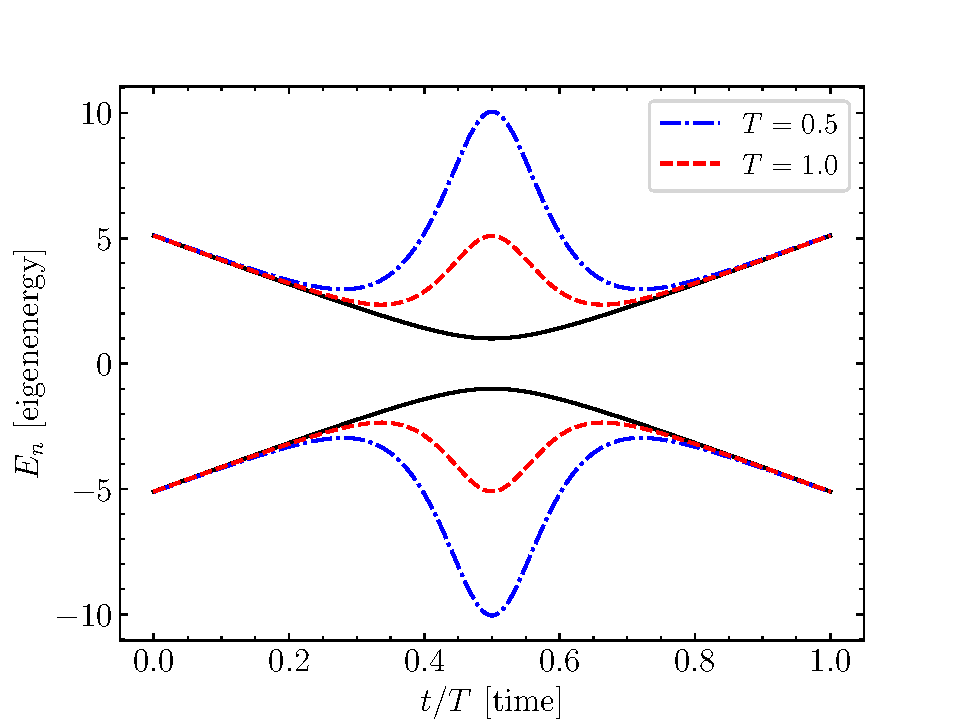
\includegraphics[width=0.5\columnwidth]{Sec2-A-IV-LZ_Energies.pdf}
\caption{Time dependence of the energy eigenvalues for the Landau-Zener model (solid, black) and for the controlled evolution, Eq.~\eqref{HCD_LZ} (dashed) for two different protocol durations assuming a linear ramp $v(t)=-5+10\tfrac{t}{T}$ and $\Delta\!=\!1$.}
\label{EnergiesHCD}
\end{figure}
For any choice of ramp, $\nu(t)$, evolving the system according to the Hamiltonian
\begin{equation}
\label{HCD_LZ}
H_\text{CD} = H + \mathcal{A} = \Delta \sigma^x + \nu(t)\sigma^z - \frac{\Delta~\partial_t \nu(t)}{2(\Delta^2 + \nu(t)^2)}\sigma^y,
\end{equation}
will ensure a perfectly adiabatic dynamics. As an example, if the system is initialised in the ground state for some initial value of the field, $\nu_0$, and we linearly ramp the system according to $\nu(t)=\nu_0+\nu_d \tfrac{t}{T}$, we can understand why this Hamiltonian achieves a perfectly adiabatic evolution by comparing the energy spectra of the original and the controlled Hamiltonians~\cite{Abah2019}. In Fig.~\ref{EnergiesHCD}, the solid curves show the behavior of the eigenenergies of the bare LZ model for a linear ramp and we clearly see the avoided crossing occurring for $t/T=0.5$. In contrast, the energy spectrum of the control Hamiltonian shows that adding the counterdiabatic term modifies the energy gap in such a way that, rather than exhibiting an avoided crossing, the energy levels are pushed apart in precisely the right manner to ensure that the rate at which the system is being driven is still slow enough, with respect to this new energy gap, that it continues to evolve adiabatically. Clearly the counterdiabatic term fundamentally changes the spectral properties of the system in order to achieve adiabaticity. Indeed, using the fact that $\mathcal{A}$ is a Hamiltonian term, several works use this as the basis for examining the thermodynamics of quantum control arguing that $\mathcal{A}$ can be thought of as a energetic toll that must be paid in order manipulate the system~\cite{ZhengPRA2016, SantosSciRep2015, CalzettaPRA2018, FunoPRL2017, AbahEPL2017, CampbellDeffnerPRL, CampbellEPL2023}. For simple models such as Eq.~\eqref{eq:LZham} it is intuitive to expect that $\mathcal{A}$ would modify the spectrum by simply opening an energy gap; however, this is not necessarily true, as has been shown by closing energy gaps in examples including non-interacting tight-binding models \cite{duncan2024exact} and many-body spin-1/2 lattice gauge models \cite{hartmann2019rapid}. In fact, the study of what constitutes the important characteristics that the counterdiabatic term induces in the spectrum of a complex many-body system is an open question. While interesting and insightful in its own right, understanding the control requirements for the LZ model is vital when moving to the genuine many-body Ising model. 
%\callum{This clear opening of the gap is not always what the AGP will implement, and we should probably point this out. I.e., while here and in some other simple or targeted examples the CD or AGP will open an energy gap, this should not be seen as required of the CD or AGP.}

\subsubsection{Example: The Ising model in 1-dimension}

The transverse field nearest-neighbor Ising model describes a collection of interacting spin-$\frac{1}{2}$ degrees of freedom on a lattice under the action of a perpendicular magnetic field. This model is often taken as an example to first consider new control protocols due to its well-known solutions and relation to other higher-complexity cases that are studied \cite{SachdevQPTs,DziarmagaPRL,Damski2006}. We will consider the 1D Ising model for simplicity, which is given by 
\begin{equation}\label{eq:Ising}
H = - \sum_{j=1}^N \left( \sigma^x_j \sigma^x_{j+1} + g \sigma_j^z\right),
\end{equation}
$\sigma_j^a$, $a \in {x,y,z} $ representing the Pauli matrix acting on the $j$-th site and $g$ the relative strength of an applied external field. This model exhibits a quantum phase transition at $g=g_c=\pm 1$ between a paramagnetic ($|g|>1$) and ferromagnetic ($|g|<1$) phase. As it is the only parameter, we will consider the scenario where $g=g(t)$, i.e., we drive $g$ and are interested in implementing CD terms such that we negate any diabatic transitions so that, e.g., we can remain in the ground state of the system in a finite driving time.

\emph{The Jordan-Wigner transformation}. It is not always possible to derive the exact CD for arbitrary Hamiltonians, but luckily the Ising model is exactly solvable through the Jordan-Wigner transformation. This allows for the exact CD to be obtained, as was done in Refs.~\cite{delCampo2012Assisted,damskiJPA2013,damskiJSM2014}. First, we will assume periodic boundary conditions, i.e. $\sigma_{N+1}=\sigma_1$, for an $N$ site system with an even number of spins and $N\geq2$. It is simpler to consider the term across the periodic boundary separately and to write the Hamiltonian as
\begin{equation}\label{eq:Isingper}
H = - \sum_{j=1}^{N-1} \sigma^x_j \sigma^x_{j+1} - \sigma^x_N \sigma^x_{1} - g  \sum_{j=1}^{N} \sigma_j^z.
\end{equation}
The Jordan-Wigner transformation is used to transform the Hamiltonian from the interacting spin basis to a basis of non-interacting fermions, and a useful summary of its implementation can be found in Refs.~\cite{mbengArXiv2020,damskiJPA2013}. We can define a set of creation and annihilation fermionic operators from the spin basis as
\begin{equation}\label{eq:JW}
c_j^\dagger = K_j^\dagger \sigma_j^-, \qquad
c_j = K_j \sigma_j^+,
\end{equation}
with
\begin{equation}
\sigma_j^\pm = \frac{1}{2}\left(\sigma_j^x \pm i \sigma_j^y\right) \qquad K_j = e^{i\pi \sum_{k<j} \sigma_k^+ \sigma_k^-} = \prod_{k<j} \left( 1 - 2 n_j \right),
\end{equation}
where $n_j=c_j^\dagger c_j$ is the number operator and $K_j$, with eigenvalues $\pm 1$, is the non-local string operator which counts the parity of the number of fermions on the lattice before site $j$. The fermionic operators obey the anti-commutation relations
\begin{equation}\label{eq:anticomm}
\left\{ c_i, c_j^\dagger \right\} = \delta_{i,j} \qquad \left\{ c_i, c_j \right\} =  \left\{ c_i^\dagger, c_j^\dagger \right\} = 0.
\end{equation}
The one-body term is then relatively straightforward as we can write the $z$-Pauli matrix on site $j$ as 
\begin{eqnarray}
\sigma_j^z & = & 1 - 2 c_j^\dagger c_j, 
\end{eqnarray}
which can be seen from
\begin{eqnarray}
\sigma_j^z & = & 1 - 2 \sigma_j^- \sigma_j^+ = 1 - \frac{1}{2}\left( \sigma_j^x - i \sigma_j^y \right) \left( \sigma_j^x + i \sigma_j^y \right) = 1 - \frac{1}{2}\left( \sigma_j^x \sigma_j^x - i^2 \sigma_j^y \sigma_j^y - i \sigma_j^y \sigma_j^x + i \sigma_j^x \sigma_j^y \right) \\ \nonumber 
& = & 1 - \frac{1}{2}\left( 1 + 1 - i [\sigma_j^y, \sigma_j^x] \right) = 1 - \left( 1 - \sigma_j^z \right) =  \sigma_j^z , 
\end{eqnarray}
note that the ordering of the Pauli matrices is important as they do not commute and we have used the fact that $[\sigma_j^y, \sigma_j^x] = -2i\sigma_j^z$. We can also write out the $x$-Pauli matrix as,
\begin{eqnarray}
\sigma_j^x & = & K_j \left( c_j^\dagger + c_j \right) \\ \nonumber
& = & K_j \left(  K_j^\dagger \sigma_j^- + K_j \sigma_j^+ \right) = \sigma_j^- + K_j K_j \sigma_j^+ = \sigma_j^- + \sigma_j^+ = \sigma_j^x,
\end{eqnarray}
where we used the fact that $K_j K_j$ acting on any state is equivalent to $\mathds{1}_j$, i.e. the identity operator. With this we can write the Ising Hamiltonian given by Eq.~\eqref{eq:Isingper} as
\begin{eqnarray}\label{eq:intermediateH}
H & = & - \sum_{j=1}^{N-1} K_j \left( c_j^\dagger + c_j \right) K_{j+1} \left( c_{j+1}^\dagger + c_{j+1} \right) - K_N \left( c_N^\dagger + c_N \right) \left( c_{1}^\dagger + c_{1} \right) - g  \sum_{j=1}^{N} \left( 1 - 2 c_j^\dagger c_j \right) \nonumber \\ 
& = & - \sum_{j=1}^{N-1} K_j K_j \left( c_j^\dagger + c_j \right) \left(1-2n_j\right) \left( c_{j+1}^\dagger + c_{j+1} \right) - K_N \left( c_N^\dagger + c_N \right) \left( c_{1}^\dagger + c_{1} \right) - g  \sum_{j=1}^{N} \left( 1 - 2 c_j^\dagger c_j \right). 
\end{eqnarray}
We can simplify this further by considering each term in turn. The first term can be written as
\begin{eqnarray}
& & - \sum_{j=1}^{N-1} K_j K_j \left( c_j^\dagger + c_j \right)  \left(1-2n_j\right)\left( c_{j+1}^\dagger + c_{j+1} \right) = - \sum_{j=1}^{N-1} \left( c_j^\dagger + c_j \right) \left(1-2 c^\dagger_j c_j\right) \left( c_{j+1}^\dagger + c_{j+1} \right) \nonumber \\
& = & - \sum_{j=1}^{N-1} \left( c_j^\dagger + c_j - 2 c_j^\dagger c^\dagger_j c_j - 2 c_j c^\dagger_j c_j \right) \left( c_{j+1}^\dagger + c_{j+1} \right) = - \sum_{j=1}^{N-1} \left( c_j^\dagger + c_j - 2 c_j \right) \left( c_{j+1}^\dagger + c_{j+1} \right) \nonumber \\
& = & \sum_{j=1}^{N-1} \left( c_j - c_j^\dagger \right) \left( c_{j+1}^\dagger + c_{j+1} \right), 
\end{eqnarray}
the second term -- as
\begin{eqnarray}
& & - K_N \left( c_N^\dagger + c_N \right) \left( c_{1}^\dagger + c_{1} \right) = - K_{N+1} \left (1-2 n_N \right) \left( c_N^\dagger + c_N \right) \left( c_{1}^\dagger + c_{1} \right) \nonumber \\
& = & - P \left( c_N^\dagger + c_N - 2 c_N^\dagger c_N c_N^\dagger - 2 c_1^\dagger c_1 c_1 \right) \left( c_{1}^\dagger + c_{1} \right) = - P \left( c_N^\dagger + c_N - 2 c_N^\dagger \right) \left( c_{1}^\dagger + c_{1} \right) \nonumber \\ & = & - P \left( c_N - c_N^\dagger \right) \left( c_{1}^\dagger + c_{1} \right), 
\end{eqnarray}
where $P=K_{N+1}$ is the parity operator for the number of fermions in the full $N$-site system. The third term cannot be simplified further, though it is common to see it written in a different form given by
\begin{equation}
\sum_{j=1}^{N} \left( 1 - 2 c_j^\dagger c_j \right) = \sum_{j=1}^{N} \left( c_j^\dagger c_j + c_j c_j^\dagger - 2 c_j^\dagger c_j \right) = \sum_{j=1}^{N} \left( c_j c_j^\dagger - c_j^\dagger c_j \right),
\end{equation}
where we have used the anti-commutation relations given in Eq.~\eqref{eq:anticomm}. All this together means we can write Eq.~\eqref{eq:intermediateH} as
\begin{equation}
H = \sum_{j=1}^{N-1} \left( c_j - c_j^\dagger \right) \left( c_{j+1}^\dagger + c_{j+1} \right) - P \left( c_N - c_N^\dagger \right) \left( c_{1}^\dagger + c_{1} \right) -g \sum_{j=1}^{N} \left( c_j c_j^\dagger - c_j^\dagger c_j \right).
\end{equation}
This Hamiltonian is invariant under the parity operator and we can therefore split it into the even parity ($P=1$) and odd parity ($P=-1$) subspaces, and write the full Hamiltonian as
\begin{equation}
H = H^+ P^+ + H^- P^-,
\end{equation}
with
\begin{equation}
P^\pm = \frac{1}{2} \left( 1 \pm P \right),~~~~\text{and}~~~~ H^\pm = \sum_{j=1}^{N} \left( c_j - c_j^\dagger \right) \left( c_{j+1}^\dagger + c_{j+1} \right) - g \sum_{j=1}^{N} \left( c_j c_j^\dagger - c_j^\dagger c_j \right), 
\end{equation}
where $H^+$ has anti-periodic boundary conditions, i.e. $c_{N+1} \equiv - c_1$, and $H^-$ has periodic boundary conditions, i.e. $c_{N+1} \equiv c_1$.

\emph{Momentum space}. We will now focus our attention on the positive parity subspace, with the consideration of the negative parity subspace being similar to the discussion below. The dynamics of the Ising spin chain given by Hamiltonian~\eqref{eq:Ising} is then described by the Schr\"odinger equation and the fermionic Hamiltonian 
\begin{equation}
H^+ = \sum_{j=1}^{N} \left( c_j - c_j^\dagger \right) \left( c_{j+1}^\dagger + c_{j+1} \right) - g \sum_{j=1}^{N} \left( c_j c_j^\dagger - c_j^\dagger c_j \right),
\end{equation}
with anti-periodic boundary conditions, $c_{N+1}=-c_1$. 

It will now be convenient to write the model in (quasi)momentum $k$-space and to do this we can first write the fermion operators in $k$-space as
\begin{equation}\label{eq:FTJW}
c_k = \frac{e^{-i \phi}}{\sqrt{N}} \sum_{j=1}^N e^{-i k j} c_j, \qquad c_j = \frac{e^{i \phi}}{\sqrt{N}} \sum_{k} e^{i k j} c_k,
\end{equation}
with the overall phase given by $\phi$ changing the phase of the pairs that will be created in $k$-space as we will see below. Note, the choice of parity subspace informs the correct values of the quasimomentum $k$. For anti-periodic boundary conditions we must satisfy $c_{N+1} \equiv - c_1$, which after transforming to $k$-space will mean $e^{i k N} = -1$, which has solutions
\begin{equation}
k = \pm \frac{\left( 2 m - 1 \right)\pi}{N} \qquad \mathrm{with} \quad m = 1,2,\dots,\frac{N}{2}.
\end{equation}
First we can Fourier transform the local term
\begin{eqnarray}
\sum_{j=1}^{N} \left( c_j c_j^\dagger - c_j^\dagger c_j \right) & = &  \frac{1}{N} \sum_j \sum_{k,k'} \left( e^{-i\left( k' - k\right)j} c_k c_{k'}^\dagger - e^{-i\left( k' - k\right)j} c_{k'}^\dagger c_k \right) \nonumber \\
& = & \sum_{k,k'} \left( \delta_{k,k'} c_k c_{k'}^\dagger - \delta_{k,k'} c_{k'}^\dagger c_k \right) = \sum_k \left( c_k c_{k}^\dagger - c_{k}^\dagger c_k \right),
\end{eqnarray}
where we have used the fact that $\delta_{m,n}=\sum_j e^{-i(n-m)j}/N$. We can follow similar steps with the nearest-neighbor term to obtain
\begin{eqnarray}
\sum_{j=1}^{N} \left( c_j - c_j^\dagger \right) \left( c_{j+1}^\dagger + c_{j+1} \right) & = & \sum_{k,k'} \left( e^{2i\phi} e^{i k'} \delta_{-k,k'} c_k c_{k'} - e^{-2i\phi} e^{-i k'} \delta_{-k,k'} c_k^\dagger c_{k'}^\dagger - \delta_{k,k'} c_{k'}^\dagger c_k + \delta_{k,k'} c_{k'} c_k^\dagger \right) \nonumber \\ 
& = & \sum_k \left( 2\cos k \; c^\dagger_k c_k + e^{2i\phi} e^{i k} c_k c_{-k} - e^{-2i\phi} e^{-i k} c_k^\dagger c_{-k}^\dagger \right),
\end{eqnarray}
where in the final step we have neglected a constant energy offset. Combining these, and using the anticommutation relations as well as the fact that $\sum_k \cos k = 0$, we can obtain the $k$-space Hamiltonian to be
\begin{equation}
H = \sum_k \left[ \left( \cos k - g\right) \left( c_k c_{k}^\dagger - c_{k}^\dagger c_{k} \right) + e^{2i\phi} e^{ik} c_k c_{-k} - e^{-2i\phi} e^{-ik} c_k^\dagger c_{-k}^\dagger \right].
\end{equation}

All terms in the Hamiltonian now come in momentum pairs, $(k,-k)$, and we can define the full Hamiltonian by only considering the positive $k$ values. Let us now define a fermionic two-component spinor 
\begin{equation}
\Psi_k = \begin{pmatrix}
c_k \\ c_{-k}^\dagger
\end{pmatrix} \qquad \Psi_k^\dagger = \begin{pmatrix}
c_k^\dagger & c_{-k}
\end{pmatrix},
\end{equation}
which we can use to rewrite the Hamiltonian as
\begin{equation}
H = \sum_{k>0} H_k \qquad \mathrm{with} \quad H_k = 2 \Psi_k^\dagger \begin{pmatrix}
g - \cos k & - i e^{-2i\phi} \sin k \\
i e^{2i\phi} \sin k & - g + \cos k
\end{pmatrix} \Psi_k.
\end{equation}
We can write out the above $2\times2$ matrix in terms of a psuedo-spin as is shown in Eq.~(54) of Ref.~\cite{mbengArXiv2020}, the choice of $\phi$ then comes down to the direction of the effective magnetic field for this psuedo-spin, for the Ising model we have written the effective magnetic field of the psuedo-spin is in the $x\!-\!z$ plane which corresponds to $\phi=-\pi/4$. Taking this value of $\phi$ we can write the Hamiltonian in momentum space as
\begin{equation}
H_k = 2 \Psi_k^\dagger \left[ \left( g - \cos k \right) \sigma^z + \sin k \sigma^x \right] \Psi_k.
\end{equation}

\emph{Back to Landau-Zener}. We have now managed to decompose the 1D Ising model into a collection of independent two-level systems. Note that, under Schr\"odinger dynamics, each two-level system will undergo a Landau-Zener transition. We can now utilise the results of Sec.~\ref{sec:LandauZener}, identifying $\Delta = 2 \sin k$ and $v(t) = 2g - 2\cos k$, and the CD term can be written as
\begin{equation}
\mathcal{A} = - \sum_{k>0}  \frac{\dot{g}\sin k }{2\left( 1 + g^2 - 2g\cos k \right)} \Psi_k^\dagger \sigma^y \Psi_k.
\end{equation}
If one is only interested in being able to numerically calculate the outcome of a protocol with CD this is where we could stop. However, while we have the CD term in a nice form, expressing this in $k$-space may not be ideal for physical implementation. In addition, as the CD term is local in $k$-space, we should expect that it will be highly non-local in physical space; but this physical space alone is the space of the non-interacting fermions, and we must remember that the native basis for our initial Hamiltonian is in fact spin-$1/2$'s.

Having Fourier converted the problem of spin-$1/2$'s to non-interacting fermions and then transformed to $k$-space, we now find ourselves with the CD term but with the need to trek back along the path we have followed to this point. First we can write out the CD term in the fermion operators as
\begin{equation}
\mathcal{A} = - i \sum_{k>0} \frac{\dot{g}\sin k }{2\left( 1 + g^2 - 2g\cos k \right)} \left( c_k c_{-k} - c_k^\dagger c_{-k}^\dagger \right),
\end{equation}
then utilising the inverse Fourier transform defined in Eq.~\eqref{eq:FTJW} we can write this in position space as
\begin{equation}
\mathcal{A} = - \frac{i}{2N} \dot{g} \sum_{j,j'}^N \sum_{k>0} \frac{\sin k}{1 + g^2 - 2g\cos k} \sin \left( \left( j - j' \right) k \right) \left( c_j c_{j'} + c_j^\dagger c_{j'}^\dagger \right),
\end{equation}
remembering that we only need to consider positive $k$. We see that, as expected, the CD term is highly non-local in physical space as it is a sum over all pairs of sites in the 1D lattice. We can now write the CD term in terms of Pauli matrices, using Eq.~\eqref{eq:JW},
\begin{eqnarray}
\mathcal{A} & = & - \frac{i}{2} \dot{g} \sum_{j,j'}^N f\left( j - j' \right) \left( c_j c_{j'} + c_j^\dagger c_{j'}^\dagger \right) \nonumber \\
& = &  - \frac{i}{2} \dot{g} \sum_{j,j'}^N f\left( j - j' \right) \left[ K_j K_j \sigma_j^+ \left( \prod_{j \leq m < j'}  \sigma_m^z \right) \sigma_{j'}^+ +  K_j^\dagger K_j^\dagger \sigma_j^- \left( \prod_{j \leq m < j'}  \sigma_m^z \right) \sigma_{j'}^- \right] \nonumber \\
& = & - \dot{g} \sum_{j,j'}^N f\left( j - j' \right) \left[ \sigma_j^y \left( \prod_{j < m < j'}  \sigma_m^z \right) \sigma_{j'}^x + \sigma_j^x \left( \prod_{j < m < j'}  \sigma_m^z \right) \sigma_{j'}^y \right],
\label{eq:HCDIsing}
\end{eqnarray}
where in the last step we have removed a $\sigma_j^z$ from the product and used the fact that $\sigma^x_j \sigma_j^z = - i \sigma_j^x$ and $\sigma_j^y \sigma_j^z = i \sigma_j^x$. 

Achieving perfect control still requires knowledge of the coefficients, $f(j-j')$, the precise determination of which is highly non-trivial~\cite{delCampo2012Assisted, damskiJSM2014}, as we will discuss explicitly shortly. Nevertheless, Eq.~\eqref{eq:HCDIsing} is the exact CD term for the 1D Ising model in the native spin-$1/2$ basis. As anticipated, it is a highly non-local operator which couples spins across the full system and, in this regard, it is instructive to examine how the complexity of the CD term emerges as we scale up the size of the system. For $N\!=\!2$ we can directly compute the exact $\mathcal{A}$ using Eq.~\eqref{HCD} and find
\begin{equation}
\mathcal{A} \propto \left(\sigma^y_1\sigma_2^x + \sigma^x_1\sigma_2^y \right)
\end{equation}
similarly for $N=3$ 
\begin{equation}
\mathcal{A}\propto\left( \sigma^y_1\sigma_2^x + \sigma^x_1\sigma_2^y + \sigma^y_2\sigma_3^x + \sigma^x_2\sigma_3^y + \sigma^y_3\sigma_1^x + \sigma^x_3\sigma_1^y\right).
\end{equation}
where we see the operators entering the control terms are precisely those appearing in Eq.~\eqref{eq:HCDIsing}. Thus, while Eq.~\eqref{eq:HCDIsing} provides the overall form of the counterdiabatic term, it still remains to determine the correct form of the coefficients, $f(j-j')$. For $N=2$ it is easy to find the explicit form of the coefficient by direct calculation, resulting in the CD term taking the compact form
\begin{equation}
\mathcal{A} =-\frac{\dot{g}}{4(1+g^2)} \left(\sigma^y_1\sigma_2^x + \sigma^x_1\sigma_2^y \right).
\end{equation}
Already determining the precise coefficients even for $N=3$ becomes significantly more involved; however, if we restrict to only controlling the ground state we find by direct calculation
\begin{equation}
A_\text{GS}= -\dot{g}\frac{1 + g}{8(1+g^3)}\left( \sigma^y_1\sigma_2^x + \sigma^x_1\sigma_2^y + \sigma^y_2\sigma_3^x + \sigma^x_2\sigma_3^y + \sigma^y_3\sigma_1^x + \sigma^x_3\sigma_1^y\right),
\end{equation}
where the choice of symbol reflects the fact that, despite the operators appearing in $A_\text{GS}$ corresponding precisely to those that make up $\mathcal{A}$, the choice of coefficients means that this counterdiabatic term will not suppress excitations for all eigenstates of the Hamiltonian. In general, one can take a similar approach to Ref.~\cite{delCampo2012Assisted} and assume an ansatz form for the coefficients. If we restrict to control of the ground state for an even size chain with periodic boundary conditions, then we can use the results of Ref.~\cite{damskiJSM2014}, which provides an analytic form for the coefficients. For consistency with Refs.~\cite{delCampo2012Assisted, damskiJSM2014} we slightly rearrange Eq.~\eqref{eq:HCDIsing} into the form
\begin{equation}
\label{eq:HCDIsing2}
A_\text{GS}=-\dot{g} \left[\sum_{m=1}^{N/2-1} h_{m}(g) A_\text{GS}^{[m]} + \frac{1}{2}h_{N/2}(g) A_\text{GS}^{[N/2]} \right]    
\end{equation}
where the coefficients are now given precisely by
\begin{equation}
h_m(g) = \frac{g^{2m}+g^N}{8g^{m+1}(1+g^N)}.
\end{equation}
It should be clear that each $m$ term in Eq.~\eqref{eq:HCDIsing2} corresponds to a different ``range'' of interactions given by
\begin{equation}
A_\text{GS}^{[m]} = \sum_{n=1}^{N} \left[ \sigma^y_n \left( \prod_{j=n+1}^{n+m-1} \sigma^z_j \right) \sigma^x_{n+m} + \sigma^x_n \left( \prod_{j=n+1}^{n+m-1} \sigma^z_j \right) \sigma^y_{n+m} \right],
\end{equation}
with $m=1$ corresponding to nearest neighbor terms, i.e. no $\sigma^z_j$'s appearing as e.g. seen in the $N=2$ and 3 cases, and we extend up to a maximal range of $N/2$ due to the assumed periodic boundary conditions. Note that the factor of $1/2$ appearing in front of $A_\text{GS}^{[N/2]}$ is due to the even system size which results in there being only a single spin at the ``maximal" distance of $N/2$ from site 1. 
%\marin{something's wrong with this sentence but it's not completely clear what u wanted to say so I can't fix it w/o losing on content; better split in parts}\steve{clearer now?}
%%%%%%%%%%%%%%%%%%%%%%%ISING FIGURE%%%%%%%%%%%%%%%%%%%%%%%%%
\begin{figure}[t]
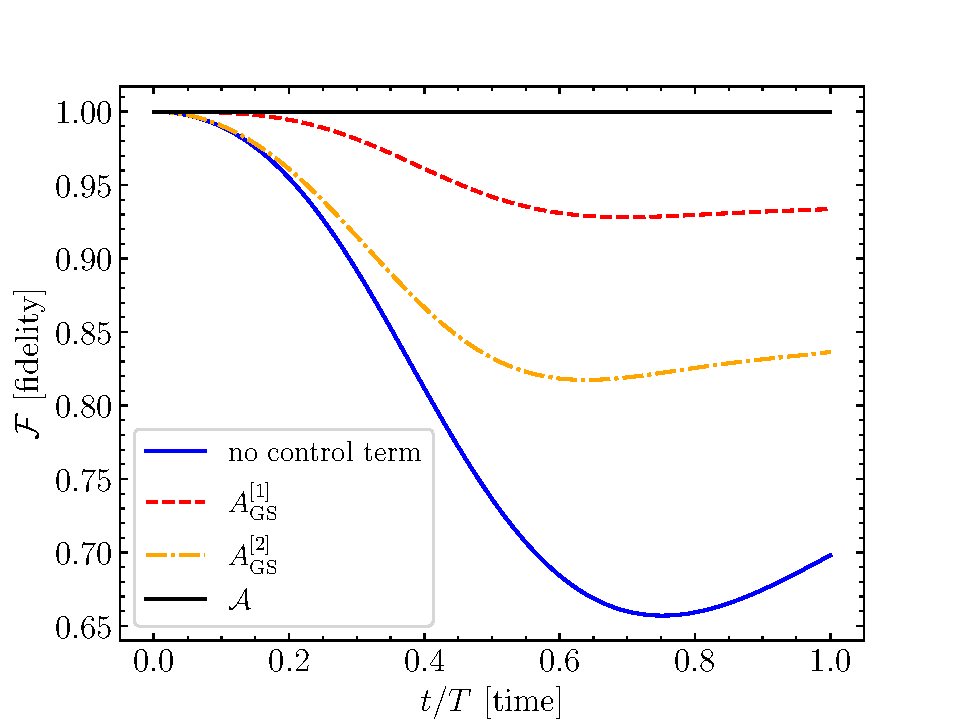
\includegraphics[width=0.5\columnwidth]{Sec2-A-V-IsingFigure.pdf}
\caption{Ising model for $N=4$ with $g(t)=0.1+1.9 t/T$ fixing $T \!=\!1$ and starting in the ground state. We show the fidelity with the instantaneous ground state for the full counterdiabtic term (black) involving all two and three body interactions i.e. Eq.~\eqref{eq:HCDIsingFull}, implementing only the two-body terms i.e. Eq.~\eqref{eq:HCDIsing2body} (dashed, red), implementing only the three-body terms i.e. Eq.~\eqref{eq:HCDIsing3body} (dot-dashed, orange). We also show the evolution for the bare Hamiltonian (blue).}
\label{IsingFig}
\end{figure}
%%%%%%%%%%%%%%%%%%%%%%%ISING FIGURE%%%%%%%%%%%%%%%%%%%%%%%%%
This allows us to write out explicitly the control term that will maintain adiabatic dynamics for the ground state for $N=4$, which is the smallest system size such that there are contributions arising from both terms in Eq.~\eqref{eq:HCDIsing2} with 
\begin{eqnarray}
A_\text{GS} = A_\text{GS}^{(2)} &=& -\dot{g} \left[ h_1(g) A_\text{GS}^{[1]} + \frac{1}{2} h_2(g) A_\text{GS}^{[2]}  \right]~~\text{where} \label{eq:HCDIsingFull} \\
h_1(g) A_\text{GS}^{[1]} &=& \frac{1 + g^2}{8(1+g^4)} \left( \sigma^y_1\sigma_2^x + \sigma^x_1\sigma_2^y + \sigma^y_2\sigma_3^x + \sigma^x_2\sigma_3^y+ \sigma^y_3\sigma_4^x + \sigma^x_3\sigma_4^y + \sigma^y_4\sigma_1^x + \sigma^x_4\sigma_1^y \right) \label{eq:HCDIsing2body} \\ 
h_2(g) A_\text{GS}^{[2]} &=&  \frac{g}{4(1+g^4)} \left( 
\sigma^y_1\sigma_2^z\sigma_3^x + \sigma^x_1\sigma_2^z\sigma_3^y + 
\sigma^y_2\sigma_3^z\sigma_4^x + \sigma^x_2\sigma_3^z\sigma_4^y +
\sigma^y_3\sigma_4^z\sigma_1^x + \sigma^x_3\sigma_4^z\sigma_1^y +
\sigma^y_4\sigma_1^z\sigma_2^x + \sigma^x_4\sigma_1^z\sigma_2^y\right) \label{eq:HCDIsing3body}
\end{eqnarray}
where for consistency of notation with Sec.~\ref{subsec:varl_AGP} we introduce $A_\text{GS}^{(m)}$ to denote the cumulative control term utilising all interactions with ranges up to and including $m$-body terms, i.e. the sum of the individual terms with a specific range $A_\text{GS}^{[m]}$. In Fig.~\ref{IsingFig} we show the relevance of the different contributions in achieving control of the full system. We see that if we include only the two-body control terms, i.e. evolve according to $H-\dot{g}h_1(g)A_\text{GS}^{[1]}$, these terms provide the most significant improvement in the ability control of the system when compared to the performance if we include only the three body control terms, i.e. evolve according to $H-\dot{g}h_2(g)A_\text{GS}^{[2]}$. Clearly, given that we are considering only $N\!=\!4$, perfect control is achieved when both two- and three-body terms are present and the system is evolved under $H+A_\text{GS}^{(2)}$. 
%in Fig.~\ref{IsingFig} \marin{I'm confused: $\mathcal{A}^{[2]}$ curve is not unit fidelity, so why perfect ctrl? Why show separate terms and not the cumulative sum in Fig 3?} \callum{I believe $\mathcal{A}^{[2]}$ is only that one, and the unit fidelity is with $\mathcal{A}$}.

\subsubsection{Example: The Ising model with all-to-all couplings (Lipkin-Meshkov-Glick model)}
\label{ex:LMGmodel}
While the previous section considered the solvable Ising model with nearest neighbor interactions, for which the exact CD term for any $N$ can be determined, we can also look at a complementary interaction setting, where all constituents mutually interact with one-another. This all-to-all coupling, or infinite range interaction, is captured by the Lipkin-Meshkov-Glick (LMG) Hamiltonian
\begin{equation}\label{eq:LMG}
H = - \frac{1}{N}\sum_{j<k}^N \sigma^x_j \sigma^x_{k} -\sum_j^N g(t) \sigma_j^z.
\end{equation}
Originally proposed as a model to study shape phase transitions in atomic nuclei, Eq.~\eqref{eq:LMG} has since come to encompass a wide range of physical phenomena including as a model of magnetism~\cite{LMG1, LMG2} and as a paradigmatic model for studying quantum phase transitions~\cite{ESQPTreview}. Notice that unless warranted for clarity, we use $g(t)\equiv g$ for brevity.

From the quantum many-body perspective, this model is interesting due to its very rich phase diagram, host to ground and excited state quantum phase transitions thanks to the high degree of symmetry the all-to-all interaction provides. In the thermodynamic limit, $N\to \infty$, the ground state phase transition is between symmetric ($0\!<\!g\!<\!1$) and symmetry broken ($g\!>\!1$) phases. In the symmetric phase, even and odd parity subspaces are degenerate (and quasi-degenerate for large but finite $N$ with the gap between even and odd sub-sector energies inversely scaling with system size), while in the symmetry broken phase this degeneracy is lifted~\cite{LMG1, FazioLMG}. Despite the similarities with the Ising model, while Eq.~\eqref{eq:Ising} can be solved for arbitrary values of $N$ the same is not true for Eq.~\eqref{eq:LMG}. However, due to the high degree of symmetry that this Hamiltonian exhibits, it is more amenable to a mean-field type approach, allowing for the model to be exactly solvable in the thermodynamic limit by mapping to a quantum harmonic oscillator. This raises interesting consequences when aiming to achieve control of the model: tools and techniques have been developed to control a harmonic oscillator~\cite{MugaJPB}; that said, clearly for any finite $N$ the mapping will only be an approximation and therefore leaves questions as to the efficacy of ``naively'' applying such control approaches. To examine this, however, we must first solve the model. In what follows we will focus on the symmetry broken phase only, i.e. $g>1$, carefully detailing the steps necessary to find the solution. An almost identical calculation can be performed for the symmetric phase, with some caveats that we will discuss later and details of which can be found in, e.g. Ref.~\cite{TakahashiPRE}. 

The first step is to exploit the symmetry induced by the homogeneous all-to-all interactions. This means that it is more convenient to write Eq.~\eqref{eq:LMG} using collective spin operators, $S_\alpha = \tfrac{1}{2}\sum_n \sigma^\alpha_n$ giving
\begin{equation}
\label{eq:LMGcoll}
H= -\frac{2}{N} S_x^2 -2g S_z + \frac{1}{2}\mathds{1}.
\end{equation}
Notice that the last term, proportional to $\mathds{1}$, will have no impact on the dynamics that we will study, it simply amounts to a global phase, and hence is often neglected. For pedagogical reasons of completeness we will keep this term. It is easy to confirm that $\mathbf{S}^2$ is a conserved quantity and we can view the $N$-particle system as an effective $(N\!+\!1)$-level spin. 
We can solve to find the ground state of the model by mapping to {\it bosonic} operators following the Holstein-Primakoff approximation, which is valid for $N\!\gg\! 1$. If we restrict to $g\!>\! 1$, the individual spins all tend to align along the $z$ direction, and therefore we can define our collective spin operators in reference to this axis,
\begin{eqnarray}
\label{eq:HPapprox}
S_+ = \sqrt{N} a,&&\qquad S_-=\sqrt{N}a^{\dagger},\nonumber\\ 
\implies~S_x=\frac{1}{2}(S_+ + S_-),~\qquad S_y&=&\frac{1}{2i}(S_+ - S_-),~\qquad S_z=\frac{N}{2}-a^\dagger a.
\end{eqnarray}
In this picture, a state with all spins pointing up along $z$ corresponds to the vacuum, i.e. $\langle a^\dagger a \rangle=0$. Plugging these into Eq.~\eqref{eq:LMGcoll} we find
\begin{eqnarray}
H&=& -\frac{2}{N} \left( \frac{1}{4}(S_+ + S_-)(S_+ + S_-) \right) - 2 g S_z + \frac{1}{2}\mathds{1} \nonumber \\
&=& -\frac{2}{N} \left( \frac{N}{4}(a + a^\dagger)(a + a^\dagger) \right) - 2 g \left(\frac{N}{2} - a^{\dagger}a\right) + \frac{1}{2} \\
&=& -\frac{1}{2} \left( a^2 + (a^\dagger)^2 + a^\dagger a + a a^\dagger \right) - 2g \left(\frac{N}{2} - a^\dagger a \right) + \frac{1}{2},  \nonumber
\end{eqnarray}
and collecting terms together and using the canonical commutation relation, $a a^\dagger = 1+a^\dagger a$, we finally arrive at our Hamiltonian written only in terms of bosonic annihilation and creation operators
\begin{eqnarray}
H&=& -\frac{1}{2} \left(a^2 + (a^\dagger)^2 \right) - \frac{1}{2}\left( a^\dagger a + a a^\dagger \right) + 2 g a^\dagger a + \frac{1-2g N}{2} \nonumber \\
&=& -\frac{1}{2}\left(a^2 + (a^\dagger)^2 \right) + a^\dagger a \left( 2 g -1 \right) - g N. \label{eq:LMGmapped}
\end{eqnarray}
We now want to diagonalise this Hamiltonian in order to remove the difficult terms in $a^2$ and $(a^\dagger)^2$. This can be achieved using a Bogoliubov transformation. For the symmetry broken phase ($g>1$) that we are focusing on, we start by making the following transformation
\begin{eqnarray}
a &=& \sinh\left( \frac{\alpha}{2} \right) b^\dagger + \cosh\left( \frac{\alpha}{2} \right) b, \nonumber \\
a^\dagger &=& \sinh\left( \frac{\alpha}{2} \right) b + \cosh\left( \frac{\alpha}{2} \right) b^\dagger. \label{eq:BogTrans}
\end{eqnarray}
While at first sight this would seem to complicate things, we will see that it is through a judicious choice of the argument, $\alpha$, that is determined by a suitable quotient of the coefficients in Eq.~\eqref{eq:LMGmapped}, which allows us to diagonalise the model. To proceed, we require the expressions $\left(a^2+(a^\dagger)^2\right)$ and $a^\dagger a$ in terms of the new bosonic operators $b$ and $b^\dagger$:
\begin{eqnarray}
a^2&=& \left( \sinh\left( \frac{\alpha}{2} \right) b + \cosh\left( \frac{\alpha}{2} \right) b^\dagger \right)^2 \nonumber \\
&=& \sinh^2\left( \frac{\alpha}{2} \right) (b^\dagger)^2 + \cosh^2\left( \frac{\alpha}{2} \right) b^2 + \cosh\left( \frac{\alpha}{2} \right)\sinh\left( \frac{\alpha}{2} \right) \left(1+2b^\dagger b \right), \label{eq:asq}\\
(a^\dagger)^2&=& \left( \sinh\left( \frac{\alpha}{2} \right) b^\dagger + \cosh\left( \frac{\alpha}{2} \right) b \right)^2 \nonumber \\
&=& \sinh^2\left( \frac{\alpha}{2} \right) b^2 + \cosh^2\left( \frac{\alpha}{2} \right) (b^\dagger)^2 + \cosh\left( \frac{\alpha}{2} \right)\sinh\left( \frac{\alpha}{2} \right) \left(1+2b^\dagger b \right), \label{eq:adagsq}\\
\implies a^2+(a^\dagger)^2 &= & \left( \cosh^2\left( \frac{\alpha}{2} \right)+ \sinh^2\left( \frac{\alpha}{2} \right) \right)\left( b^2 + \left(b^\dagger\right)^2 \right) +2 \cosh\left( \frac{\alpha}{2} \right)\sinh\left( \frac{\alpha}{2} \right) \left(1+2b^\dagger b \right) \nonumber \\
&=& \cosh\left( \alpha \right) \left( b^2 + \left(b^\dagger\right)^2 \right) + \sinh\left(\alpha \right) \left(1+2b^\dagger b \right), \\
a^\dagger a & = & \left( \sinh\left( \frac{\alpha}{2} \right) b + \cosh\left( \frac{\alpha}{2} \right) b^\dagger \right)\left( \sinh\left( \frac{\alpha}{2} \right) b^\dagger + \cosh\left( \frac{\alpha}{2} \right) b \right) \nonumber \\
& = &  \sinh\left( \frac{\alpha}{2} \right)  \cosh\left( \frac{\alpha}{2} \right) (b^\dagger)^2 + \sinh\left( \frac{\alpha}{2} \right)  \cosh\left( \frac{\alpha}{2} \right) b^2 +\cosh^2\left( \frac{\alpha}{2} \right) b^\dagger b + \sinh^2\left( \frac{\alpha}{2} \right) \left(1+b^\dagger b\right) \nonumber \\
&= & \frac{1}{2}\sinh\left(\alpha\right) \left(b^2 + (b^\dagger)^2\right) + \cosh\left(\alpha\right) b^\dagger b + \sinh^2\left(\frac{\alpha}{2}\right),
\end{eqnarray}
where we have used the relations $\sinh(2x)=2\sinh(x)\cosh(x)$ and $ \cosh^2\left( \frac{x}{2} \right)+ \sinh^2\left( \frac{x}{2} \right) = \cosh(x) $. We therefore find the Hamiltonian, Eq.~\eqref{eq:LMGmapped}, transformed according to Eq.~\eqref{eq:BogTrans} is
\begin{equation}
\label{eq:MappedMess}
H=-\frac{1}{2} \left( \cosh\left( \alpha \right) \left( b^2 + \left(b^\dagger\right)^2 \right) + \sinh\left(\alpha \right) \left(1+2b^\dagger b \right) \right) + \left(2 g -1 \right) \left( \frac{1}{2}\sinh\left(\alpha\right) \left(b^2 + (b^\dagger)^2\right) + \cosh\left(\alpha\right) b^\dagger b + \sinh^2\left(\frac{\alpha}{2}\right) \right) - g N.
\end{equation}
While indeed apparently more complicated than our original Hamiltonian, we now make use of the special choice for the argument
\begin{equation}
\label{eq:BogArgument}
\tanh \left(\alpha\right) = \frac{1}{2g-1},
\end{equation}
which we see is related simply to the ratio of the relevant coefficients appearing in Eq.~\eqref{eq:LMGmapped}. This then allows us to write Eq.~\eqref{eq:MappedMess} solely in terms of $\sinh\left(\alpha\right)$ since 
$$\cosh \left(\alpha\right)= \frac{\sinh \left(\alpha\right)}{\tanh \left(\alpha\right)} = (2 g -1)\sinh \left(\alpha\right).$$ 
Thus, we have
\begin{eqnarray}
H&=&-\frac{1}{2} \frac{\sinh\left( \alpha \right)}{\tanh\left( \alpha \right)} \left( b^2 + \left(b^\dagger\right)^2 \right) -\frac{1}{2} \sinh\left(\alpha \right) \left(1+2b^\dagger b \right) + \frac{1}{2}\left(2 g -1 \right) \sinh\left(\alpha\right) \left(b^2 + (b^\dagger)^2\right) \nonumber \\
  &&~~~~ + \left(2 g -1 \right) \frac{\sinh\left( \alpha \right)}{\tanh\left( \alpha \right)} b^\dagger b + \left(2 g -1 \right) \sinh^2\left(\frac{\alpha}{2}\right) - g N  \nonumber \\
&=& -\frac{1}{2} \left(2 g -1\right)\sinh \left(\alpha\right) \left( b^2 + \left(b^\dagger\right)^2 \right) + \frac{1}{2}\left(2 g -1 \right) \sinh\left(\alpha\right) \left(b^2 + (b^\dagger)^2\right)  -\frac{1}{2} \sinh\left(\alpha \right) \left(1+2b^\dagger b \right) \nonumber \\
        &&~~~~     + \left(2 g -1 \right)  (2 g -1)\sinh \left(\alpha\right) b^\dagger b + \left(2 g -1 \right) \sinh^2\left(\frac{\alpha}{2}\right) - g N,
\end{eqnarray}
where we now see that the terms involving $b^2$ and $(b^\dagger)^2$ cancel and, after a little algebra to collect together terms such that we can express $H$ in the standard harmonic oscillator form, we are left with
\begin{equation}
H=\left( 4g^2 -4g \right) \sinh \left(\alpha\right) \left(b^\dagger b + \frac{1}{2}\right) - g\left(N+1\right) +\frac{1}{2}.
\end{equation}
From Eq.~\eqref{eq:BogArgument} it follows that $\sinh \left(\alpha\right) = \left( 4 g^2 - 4g \right)^{-1/2}$, finally giving us our desired mapped Hamiltonian
\begin{equation}
\label{eq:LMGho}
H = 2\sqrt{g(g-1)} \left(b^\dagger b + \frac{1}{2} \right) - g(N+1) + \frac{1}{2}.
\end{equation}

The reason for doing this is that the precise form for the counterdiabatic term is known in the case of a quantum harmonic oscillator~\cite{MugaJPB} with a time dependent frequency, $\omega$, and is given by
\begin{equation}
\label{eq:CDqho}
\mathcal{A} = i \frac{\dot \omega}{4\omega} \left( b^2 - (b^\dagger)^2 \right).
\end{equation}
From Eqs.~\eqref{eq:asq} and \eqref{eq:adagsq} we see that
\begin{eqnarray}
a^2-a^{\dagger2} &=&  \left(\cosh^2\left(\frac{\alpha}{2}\right) - \sinh^2\left(\frac{\alpha}{2}\right) \right) b^2 + \left(\sinh^2\left(\frac{\alpha}{2}\right) - \cosh^2\left(\frac{\alpha}{2}\right) \right) b^{\dagger2} \nonumber \\
&=& b^2-b^{\dagger2}.
\end{eqnarray}
Therefore we can readily determine the operators that the counterdiabatic term depends on in the collective spin picture by simply reverting using Eq.~\eqref{eq:HPapprox}
\begin{eqnarray}
A_\text{GS} &\propto& \frac{1}{N} \left(S_+^2 - S_-^2 \right) \label{eq:propto} \\
 &=& \frac{1}{N}\left( \left(S_x+i S_y\right)^2 -  \left(S_x+i S_y\right)^2 \right) \nonumber \\
 &=& \frac{2i}{N}\left( S_xS_y + S_yS_x \right). \nonumber
\end{eqnarray}
The counterdiabatic term for the ground state of LMG model then follows by identifying the frequency, $\omega=2\sqrt{g(g-1)}$, where we remind that $g$ is the time-dependent parameter. We therefore finally find that the control term for $g>1$ is given by
\begin{equation}
\label{eq:LMGCDterm}
A_\text{GS} = -\frac{\left(2 g -1 \right) \dot g}{4N g\left(g-1 \right)} \left( S_xS_y + S_yS_x \right).
\end{equation}
We again stress that due to the regime of validity of the Holstein-Primakoff approximation, this term is an approximation for any finite $N$ and only strictly applies to the ground state; nevertheless, it provides useful insight insofar as it indicates the operators that are likely to be highly relevant in achieving control over the system. As it is an approximation, it is prudent to test its effectiveness. For a ramp restricting to the symmetry broken phase, taking $g(t)=g_0+g_d \frac{t}{T}$ we show in Fig.~\ref{LMGfig}(a) the performance, as determined by the final target state fidelity, of this ramp as we increase system size. For comparison we show unitary dynamics with no counterdiabatic driving term (blue) and the exact, numerically calculated counterdiabatic term (black), i.e. Eq.~\eqref{HCD} evaluated explicitly for the finite sized system. We clearly see that since Eq.~\eqref{eq:LMGCDterm} is an approximation it does not perfectly suppress the non-adiabatic transitions. However, crucially we see its performance improve as we increase the system size (notice that the apparent plateauing behavior is discussed by Takahashi~\cite{TakahashiPRE}). 

\begin{figure}[t]
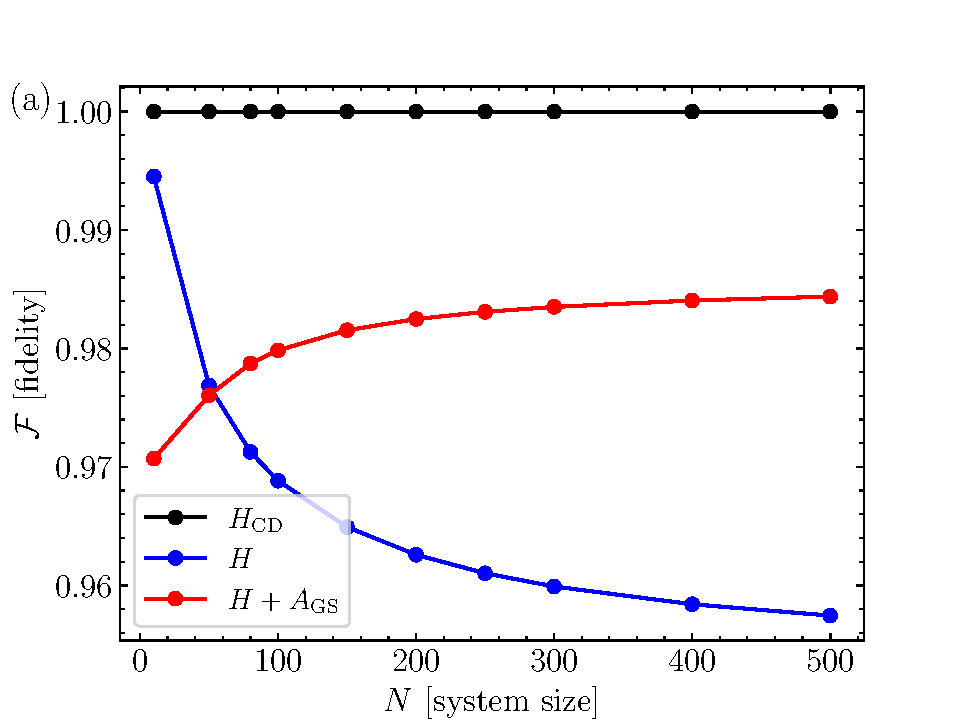
\includegraphics[width=0.49\columnwidth]{LMG_plot1.pdf}
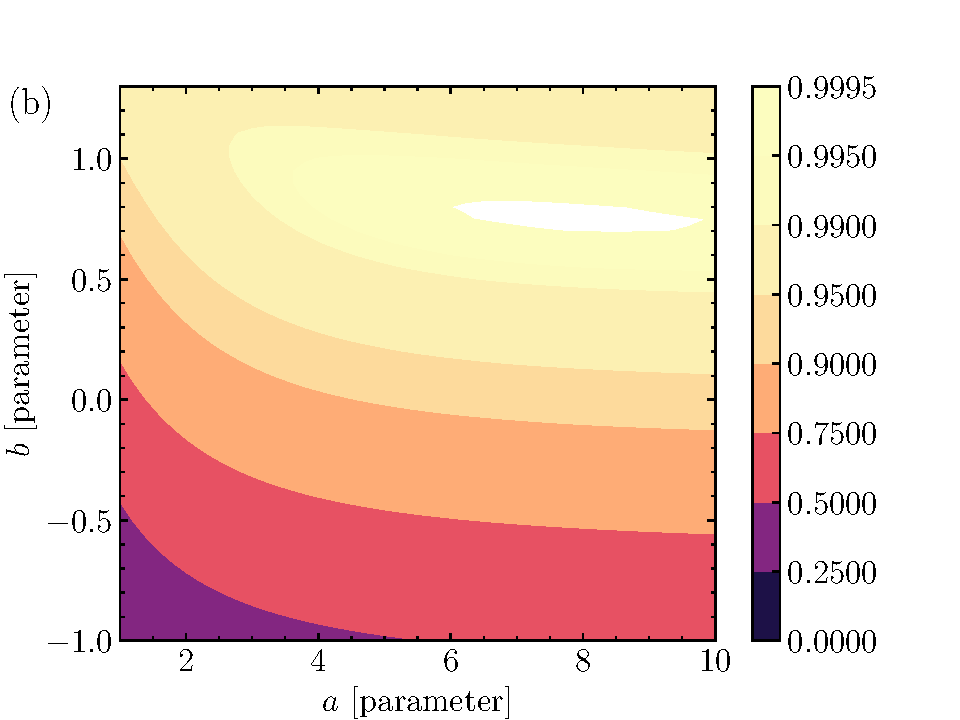
\includegraphics[width=0.49\columnwidth]{LMG_plot2.pdf}
\caption{(a) Ramping within the symmetry broken phase of the all-to-all model, with $g(t)=2-0.9 t$ where the aim is to connect the ground state of $H$ at $t=0$ with the ground state at $t=1$. We show the final target state fidelity at $t=1$ as a function of system size for the exact, numerically evaluated CD (black), bare evolution (blue), and using the QHO approximation, Eq.~\eqref{eq:LMGCDterm}, (red). (b) We fix $N=50$ and use the guess pulse Eq.~\eqref{eq:GuessPulseLMG} for the control given by the QHO approximation and sweep over the achievable fidelities.}
\label{LMGfig}
\end{figure}

Given that Eq.~\eqref{eq:LMGCDterm} is an approximation, it leaves open the question as to whether we can do better by leveraging the information we have learned from the mapping, specifically the choice of operators that enter the control term, and examine whether there is a better choice for the driving profile. 
%\marin{One thing that is often underappreciated about CD driving is that it is insensitive to the form of the drive protocol; however, whenever CD driving is approximate, different protocols will deviate from perfect transitionless driving in their own way. Therefore, one may wonder whether an improved fidelity can be achieved by suitably choosing the drive protocol $g(t)$.}
As a simple demonstration of this concept, somewhat inline with Ref.~\cite{CampbellPRL}, we consider the functional form of the coefficient in front of the operators in Eq.~\eqref{eq:LMGCDterm}. We can replace this with a simple pulse with a similar profile
\begin{equation}
\label{eq:GuessPulseLMG}
f(t) = \frac{\exp(t^a)-b}{N}.
\end{equation}
The task is then to determine what combination of the parameters $a$ and $b$ will give the best final state fidelity while still assuming the same ramping profile for $g(t)$, i.e. the linear protocol. For this simple case, we show the landscape in Fig.~\ref{LMGfig}(b) where we consider a fixed system size, $N=50$. We see that remarkably high target fidelities can be achieved. While the choice of pulse here was for ease of demonstration, it is clear that this hybrid approach is one which optimal control techniques are particularly suited to, especially if we allow for a more general pulse profile. 

While the above analysis holds for the symmetry broken phase, $g>1$, a qualitatively similar calculation can be done for the symmetric phase. This results in a control Hamiltonian with the same general form as Eq.~\eqref{eq:LMGCDterm} but with a different coefficient. In doing the mapping, the key difference is that the axis around which the Holstein-Primakoff approximation, Eq.~\eqref{eq:HPapprox}, (or equivalently the Bogoliubov transformation) is performed depends on the exact value of $g$. We refer to Refs.~\cite{TakahashiPRE, CampbellPRL, LMG1, LMG2} for more details. A remark regarding the simulation of the model in the symmetric phase: due to the quasi-degeneracy of the different parity sub-sectors, care must be taken when numerically implementing the control since the small energy gaps can lead to numerical instabilities in the dynamics. 

The above example demonstrates a key message of the present tutorial: hybrid approaches to control offer a powerful framework to coherently manipulate complex quantum systems. In particular, we see that the $N\to \infty$ limit serves as a good approximation for sufficiently large systems that we can use the functional form that the exact control term predicts and supplement it with optimal control techniques to achieve almost perfect performance. Naturally, one could have directly examined the problem from an optimal control stand point following e.g. Ref.~\cite{KochEPJQT2015}, dictating from the outset what operators to include in the control Hamiltonian and then seeking the best pulse, and for a model as relatively simple as Eq.~\eqref{eq:LMG} this would be feasible. The advantage of the above approach however is that it allows us to immediately see why a particular subset of operators are important in suppressing non-adiabatic transitions, a point that will be again explored in the next example.

The Ising and LMG models demonstrate that the exact CD terms for many-body systems necessitate non-local interactions. While some non-local interactions can be tuned in some systems, e.g. atoms coupled to cavity modes~\cite{Vaidya2018Tunable}, clearly there is an extremely high overhead in terms of the control needed over various ranges of interactions to implement the counterdiabatic term, cf. Eq.~\eqref{eq:HCDIsing} for the Ising model. In general, we find that interaction ranges necessary to achieve exact CD driving are not fixed and can be of higher order than the terms in the bare Hamiltonian. Indeed, this is the case with the Ising model in Eq.~\eqref{eq:HCDIsing}: when we map the non-local two-body terms obtained for spinless fermions back to the spin-1/2 basis, we find that we generate $N/2$-body terms with periodic boundaries and $N$ being the system size~\cite{delCampo2012Assisted}. While one approach to tackle this issue is to come up with new and novel ways in which to realise exact CD, e.g. by shaking the system in a particular way~\cite{Claeys2019Floquet}, another is to ask how important such long-range terms truly are, cfr. the discussion around Fig.~\ref{IsingFig}. In most scenarios, especially when keeping away from critical points, to obtain a substantial speed-up through a CD control protocol \steve{it} may be sufficient to consider only local approximations of the exact CD~\cite{COLD_PRXQ, Saberi2014}. In scenarios where it is possible to derive the exact counterdiabatic Hamiltonian then it is possible to take truncations of this in a sensible manner by considering dominant terms or taking a finite cut-off in the range of the exactly derived counterdiabatic terms, as demonstrated in Ref.~\cite{COLD_PRXQ} for the Ising model wherein it is shown that the variational adiabatic gauge potential provides the most insightful way to construct the control term. We next demonstrate this while also showing how the variational approach can be utilised for non-integrable models.

\subsubsection{Example: Variational counterdiabatic driving}
\label{subsec:varl_AGP}

The exact CD driving approach is powerful when feasible but limited in two central ways: {\it (i)} it requires the instantaneous Schr\"odinger equation to be solvable at all times of a given protocol, and {\it (ii)} it often results in a highly demanding non-local driving term to be implemented which can be beyond the capabilities of the hardware. The approach of variational CD driving and the use of the AGP, as detailed in Sec.~\ref{sec:varcd} was introduced in order to tackle both of these limitations at the cost of constructing only an approximate CD term.

We will take as an example the 1D Ising model, but will also include terms to make it non-integrable so that the Hamiltonian is given by
\begin{eqnarray}\label{eq:IsingNonIntegrable}
    H_0(\lambda) = -J(\lambda) \sum_j \sigma^z_j \sigma^z_{j+1} - Z(\lambda) \sum_j \sigma^z_j + X(\lambda) \sum_j \sigma^x_j,
\end{eqnarray}
with $\lambda$ being the time-dependent driving field. In this example, we will consider in detail the case of periodic boundary conditions for $N > 2$, however, we will outline where the boundary conditions become important and what happens in the case of $N=2$ for which we will derive the exact CD utilising the variational approach. In the limit of $N=1$ this model becomes equivalent to the Landau-Zener model considered in Sec. \ref{sec:LandauZener}.

From the commutator ansatz of Eq.~\eqref{eq:commansatz} we can find all possible operators on which the AGP can have non-zero support. However, this can be an exponentially large number of operators for an arbitrary $N$ size system. In this example, we will be interested in applying approximate CD driving up to two-body terms and we can turn to the commutator ansatz to obtain the correct set of operators for which the AGP can have support for up to this limit. Before moving further forward it is useful to write out the commutation rules 
\begin{eqnarray}
    \left[d A, B \right] & = & d \left[A, B \right] \nonumber\\
    \left[A, B + C\right] & = & \left[A, B \right] + \left[A, C\right] \nonumber\\
    \left[ A, BC \right] & = & B \left[ A, C \right] +  \left[ A, B \right] C \nonumber\\
    \left[ AB, C \right] & = & A \left[ B, C \right] +  \left[ A, B \right] B
\end{eqnarray}
with $A,B,C$ being operators and $d$ a scalar. Since they will be heavily used in the following, we explicitly state the commutator relations for the Pauli matrices
\begin{eqnarray}
    \left[ \sigma_j^x, \sigma_k^y \right] & = & 2 i \sigma_j^z \delta_{j,k} \nonumber \\
    \left[ \sigma_j^y, \sigma_k^z \right] & = & 2 i \sigma_j^x \delta_{j,k}  \nonumber \\
    \left[ \sigma_j^z, \sigma_k^x \right] & = & 2 i \sigma_j^y \delta_{j,k} \nonumber \\
    \left[ \sigma_j^z, \sigma_k^z \right] = \left[ \sigma_j^x, \sigma_k^x \right] & = & \left[ \sigma_j^y, \sigma_k^y \right] = 0
\end{eqnarray}
with $\delta_{j,k}$ the Kronecker delta, both of which we will use frequently in this example. We start by considering the first term of the commutator expansion, where we will drop the $\lambda$-dependence of each parameter for ease of reading,
\begin{eqnarray}
    A_\lambda^{(1)} = i \alpha_1 \left[ H_0(\lambda), \partial_\lambda H_0(\lambda) \right] & = & i \alpha_1 \sum_{j,k} \left( - J \dot{X} \left[ \sigma_j^z \sigma_{j+1}^z , \sigma_k^x \right] - Z \dot{X} \left[ \sigma_j^z, \sigma_k^x \right] - X \dot{J} \left[ \sigma_j^x, \sigma_k^z \sigma_{k+1}^z \right] - X \dot{Z} \left[ \sigma_j^x, \sigma_k^z \right] \right) \nonumber \\
    & = & i \alpha_1 \sum_{j,k} \left( \left( X \dot{J} - J \dot{X} \right) \left( \sigma_j^z \left[ \sigma_{j+1}^z, \sigma_k^x  \right] + \left[ \sigma_{j}^z, \sigma_k^x  \right] \sigma_{j+1}^z  \right) + \left( X \dot{Z} - Z \dot{X}  \right) \left[ \sigma_j^z, \sigma_k^x  \right]  \right) \nonumber \\
    & = & -2 \alpha_1 \sum_{j} \left( \left( X \dot{J} - J \dot{X} \right) \left( \sigma_j^z \sigma_{j+1}^y + \sigma_j^y \sigma_{j+1}^z  \right) + \left( X \dot{Z} - Z \dot{X}  \right) \sigma_j^y  \right) \ . \label{eq:CommutatorIsing}
\end{eqnarray}
Now we want to utilise only the information about what operators can be generated by the commutator ansatz up to two body terms. As a result, we will not utilise the coefficients derived in front of said operators and from Eq.~\eqref{eq:CommutatorIsing} we would write the ansatz for the AGP as
\begin{equation}
    A_\lambda^{(1)} = \alpha \sum_j \sigma_j^y + \gamma \sum_j \left( \sigma_j^z \sigma_{j+1}^y + \sigma_j^y \sigma_{j+1}^z  \right) \ ,
\end{equation}
with $\alpha$ and $\gamma$ being the coefficients we aim to determine. The next step would be to derive the second term of the commutator expansion, but since we are only interested in up to two body terms and the calculation of the second term is tedious, we will simply quote the result by stating that the full ansatz for the AGP including up to two-body terms is given by
\begin{equation}
    A_\lambda^{(2)} = \alpha \sum_j \sigma_j^y + \beta \sum_j \left( \sigma_j^x \sigma_{j+1}^y + \sigma_j^y \sigma_{j+1}^x  \right) + \gamma \sum_j \left( \sigma_j^z \sigma_{j+1}^y + \sigma_j^y \sigma_{j+1}^z  \right) \ ,
\end{equation}
where we also now need to find $\beta$. For comparison, we will write the ansatz for the AGP up to one-body terms as
\begin{equation}
    A_\lambda^{(1)} = \alpha \sum_j \sigma_j^y \ ,
\end{equation}
and note that the $\alpha$ coefficients for the one-body and two-body terms are not necessarily equivalent.

We now need to derive the distance we will minimise according to Sec.~\ref{sec:varcd}, first, we need to obtain $G_\lambda(A_\lambda^{(2)})$
\begin{eqnarray} \label{eq:GlambdaIsingStart}
    G_\lambda(A_\lambda^{(2)}) & = & \partial_\lambda H_0 + i \left[ A_\lambda^{(2)}, H_0 \right] \nonumber \\  & = & - \dot{J} \sum_j \sigma_j^z \sigma_{j+1}^z - \dot{Z} \sum_j \sigma_j^z + \dot{X} \sum_j \sigma_j^x + i \alpha \sum_{j,k} \left[ \sigma_j^y, - \dot{J} \sigma_k^z \sigma_{k+1}^z - \dot{Z} \sigma_k^z + \dot{X}  \sigma_k^x  \right] \nonumber \\ & & + i \beta \sum_{j,k} \left[ \sigma_j^x \sigma_{j+1}^y + \sigma_j^y \sigma_{j+1}^x, - \dot{J} \sigma_k^z \sigma_{k+1}^z - \dot{Z} \sigma_k^z + \dot{X}  \sigma_k^x  \right] + i \gamma \sum_{j,k} \left[ \sigma_j^z \sigma_{j+1}^y + \sigma_j^y \sigma_{j+1}^z, - \dot{J} \sigma_k^z \sigma_{k+1}^z - \dot{Z} \sigma_k^z + \dot{X}  \sigma_k^x  \right] \ .
\end{eqnarray}
At this point, it is useful to consider each one of the commutators in turn and we will look at each of these in the order they are presented above. Starting with the one corresponding to $\sigma^y_j$,
\begin{eqnarray}
    i \alpha \sum_{j,k} \left[ \sigma_j^y, - \dot{J} \sigma_k^z \sigma_{k+1}^z - \dot{Z} \sigma_k^z + \dot{X}  \sigma_k^x  \right] & = & i \alpha \sum_j \left( -J \sum_k \left( \sigma_k^z \left[ \sigma_j^y, \sigma_{k+1}^z \right] + \left[ \sigma_j^y, \sigma_{k}^z \right] \sigma_{k+1}^z \right) - Z \sum_k \left[ \sigma_j^y, \sigma_k^z \right] + X \sum_k \left[ \sigma_j^y, \sigma_k^x \right] \right) \nonumber \\ & = & i \alpha \sum_j \Bigg( -J \sum_k \left( \sigma_k^z \sigma_j^x \delta_{j,k+1} \left(2i\right) + \sigma_j^x \delta_{j,k} \left(2i\right)  \sigma_{k+1}^z \right) - Z \sum_k \left(2i\right) \delta_j,k \sigma_j^x + X \sum_k \left(-2i\right) \delta_j,k \sigma_j^z \Bigg) \nonumber \\ & = & 2 J \alpha \sum_j \left( \sigma_k^z \sigma_j^x + \sigma_j^x \sigma_{k+1}^z \right) + 2Z \alpha \sum_j \sigma_j^x + 2X \alpha \sum_j \sigma_j^z \ . \label{eq:Y}
\end{eqnarray}
Note that above, and in other places in the derivation of this example we use a subtle trick of labelling, the use of which can be frustrating for those who are not aware of it. For two operators labelled by $j$ and $k$, where $j$ and $k$ are summed independently over the same values, then we can always swap $j$ and $k$. This can be seen in a simple example
\begin{equation}
    \sum_{j,k} \left( A_j B_k +  A_k B_j \right) = \sum_{j,k} \left( A_j B_k +  A_j B_k \right) = 2 \sum_{j,k} A_j B_k \ ,
\end{equation}
while this trick is rather obvious when stated so bluntly, it is surprising how amid long analytical derivations such a trick can be missed, and how software, e.g., Mathematica and Maple, can not easily implement this in general. 

We now look at the commutator corresponding to $\sigma_j^x \sigma_{j+1}^y$ terms, which is rather involved, and requires the application of the commutation relation rules many times over. To start, we expand the commutator to get every term into the form of the commutation of two Pauli operators
\begin{eqnarray}
    i \beta &\sum_{j,k}& \left[ \sigma_j^x \sigma_{j+1}^y + \sigma_j^y \sigma_{j+1}^x, - \dot{J} \sigma_k^z \sigma_{k+1}^z - \dot{Z} \sigma_k^z + \dot{X}  \sigma_k^x  \right]  = \nonumber \\ 
   % & &i \beta \sum_{j} \Bigg( - J \sum_k \Big( \sigma_j^x \left[ \sigma_{j+1}^y, \sigma_k^z \sigma_{k+1}^z \right] + \left[ \sigma_{j}^x, \sigma_k^z \sigma_{k+1}^z \right] \sigma_{j+1}^y + \sigma_j^y \left[ \sigma_{j+1}^x, \sigma_k^z \sigma_{k+1}^z \right] + \left[ \sigma_{j}^y, \sigma_k^z \sigma_{k+1}^z \right] \sigma_{j+1}^x \Big) \nonumber \\
    %& &- Z \sum_k \Big( \sigma_j^x \left[ \sigma_{j+1}^y, \sigma_k^z \right] + \left[ \sigma_{j}^x, \sigma_k^z \right] \sigma_{j+1}^y + \sigma_j^y \left[ \sigma_{j+1}^x, \sigma_k^z \right] + \left[ \sigma_{j}^y, \sigma_k^z \right] \sigma_{j+1}^x \Big) + X \sum_k \left( \sigma_j^x \left[ \sigma_{j+1}^y, \sigma_k^x \right] + \left[ \sigma_{j}^y, \sigma_k^x \right] \sigma_{j+1}^x \right) \Bigg) \nonumber \\ 
    & = & i \beta \sum_{j} \Bigg( - J \sum_k \Big( \sigma_j^x \sigma_k^z \left[ \sigma_{j+1}^y, \sigma_{k+1}^z \right] + \sigma_j^x \left[ \sigma_{j+1}^y, \sigma_k^z \right] \sigma_{k+1}^z + \sigma_k^z \left[ \sigma_{j}^x, \sigma_{k+1}^z \right] \sigma_{j+1}^y + \left[ \sigma_{j}^x, \sigma_k^z \right] \sigma_{k+1}^z \sigma_{j+1}^y + \sigma_j^y \sigma_k^z \left[ \sigma_{j+1}^x, \sigma_{k+1}^z \right] \nonumber \\ 
    & &  + \sigma_j^y \left[ \sigma_{j+1}^x, \sigma_k^z \right] \sigma_{k+1}^z +  \sigma_k^z \left[ \sigma_{j}^y, \sigma_{k+1}^z \right] \sigma_{j+1}^x + \left[ \sigma_{j}^y, \sigma_k^z \right] \sigma_{k+1}^z \sigma_{j+1}^x \Big) - Z \sum_k \Big( \sigma_j^x \left[ \sigma_{j+1}^y, \sigma_k^z \right] + \left[ \sigma_{j}^x, \sigma_k^z \right] \sigma_{j+1}^y \nonumber \\ 
    & & + \sigma_j^y \left[ \sigma_{j+1}^x, \sigma_k^z \right] + \left[ \sigma_{j}^y, \sigma_k^z \right] \sigma_{j+1}^x \Big) + X \sum_k \left( \sigma_j^x \left[ \sigma_{j+1}^y, \sigma_k^x \right] + \left[ \sigma_{j}^y, \sigma_k^x \right] \sigma_{j+1}^x \right) \Bigg) .
\end{eqnarray}
We can then insert the known commutation relations and gather like terms
\begin{eqnarray}
    i \beta &\sum_{j,k}& \left[ \sigma_j^x \sigma_{j+1}^y + \sigma_j^y \sigma_{j+1}^x, - \dot{J} \sigma_k^z \sigma_{k+1}^z - \dot{Z} \sigma_k^z + \dot{X}  \sigma_k^x  \right]  = \nonumber \\ 
    & =  & i \beta \sum_{j} \Bigg( - J \sum_k \Big( \sigma_j^x \sigma_k^z \left(2i\delta_{j,k}\right) \sigma_{j+1}^x + \sigma_j^x \left(2i\delta_{j+1,k}\right) \sigma_{j+1}^x \sigma_{k+1}^z + \sigma_k^z \left(-2i\delta_{j,k+1}\right) \sigma_{j}^y \sigma_{j+1}^y + \left(-2i\delta_{j,k}\right) \sigma_{j}^y \sigma_{k+1}^z \sigma_{j+1}^y \nonumber \\ 
    & &+ \sigma_j^y \sigma_k^z \left(-2i\delta_{j,k}\right) \sigma_{j+1}^y + \sigma_j^y \left(-2i\delta_{j+1,k}\right) \sigma_{j+1}^y \sigma_{k+1}^z +  \sigma_k^z \left(2i\delta_{j,k+1}\right) \sigma_{j}^x \sigma_{j+1}^x + \left(2i\delta_{j,k}\right) \sigma_{j}^x \sigma_{k+1}^z \sigma_{j+1}^x \Big) - Z \sum_k \Big( \sigma_j^x \left(2i\delta_{j+1,k}\right) \sigma_{j+1}^x \nonumber \\ 
    & & + \left(-2i\delta_{j,k}\right) \sigma_{j}^y \sigma_{j+1}^y + \sigma_j^y \left(-2i\delta_{j+1,k}\right) \sigma_{j+1}^y + \left(2i\delta_{j,k}\right) \sigma_{j}^x \sigma_{j+1}^x \Big) + X \sum_k \left( \sigma_j^x \left(-2i\delta_{j+1,k}\right) \sigma_{j+1}^z + \left(-2i\delta_{j,k}\right) \sigma_{j}^z \sigma_{j+1}^x \right) \Bigg) \nonumber \\
    & = & 2J\beta \sum_j \left( \sigma_j^x \sigma_j^z \sigma_{j+1}^x + \sigma_j^x \sigma_{j+1}^z \sigma_{j+1}^x - \sigma_j^y \sigma_j^z \sigma_{j+1}^y - \sigma_j^y \sigma_{j+1}^z \sigma_{j+1}^y \right) + 2J\beta \sum_j \left( \sigma_j^x \sigma_{j+1}^x \sigma_{j+2}^z + \sigma_j^z \sigma_{j+1}^x \sigma_{j+2}^x - \sigma_j^z \sigma_{j+1}^y \sigma_{j+2}^y - \sigma_j^y \sigma_{j+1}^z \sigma_{j+2}^z  \right) \nonumber \\ 
    & & + 4Z\beta \sum_j \left( \sigma_j^x \sigma_{j+1}^x - \sigma_j^y \sigma_{j+1}^y \right) + 2X\beta \sum_j \left( \sigma_j^x \sigma_{j+1}^z + \sigma_j^z \sigma_{j+1}^x \right) .
\end{eqnarray}
Now, we can use the fact that we can always combine Pauli operators acting on the same site, as is present above, in this case we use that $\sigma_j^x \sigma_j^z = i \sigma_j^y$ and $\sigma_j^z \sigma_j^y = i \sigma_j^x$ to obtain
\begin{eqnarray}
     i \beta &\sum_{j,k}& \left[ \sigma_j^x \sigma_{j+1}^y + \sigma_j^y \sigma_{j+1}^x, - \dot{J} \sigma_k^z \sigma_{k+1}^z - \dot{Z} \sigma_k^z + \dot{X}  \sigma_k^x  \right]  = \nonumber \\ 
    & = & 2iJ\beta \sum_j \left( \sigma_j^y \sigma_{j+1}^x + \sigma_j^x \sigma_{j+1}^y - \sigma_j^x \sigma_{j+1}^y - \sigma_j^y \sigma_{j+1}^x \right) + 2J\beta \sum_j \left( \sigma_j^x \sigma_{j+1}^x \sigma_{j+2}^z + \sigma_j^z \sigma_{j+1}^x \sigma_{j+2}^x - \sigma_j^z \sigma_{j+1}^y \sigma_{j+2}^y - \sigma_j^y \sigma_{j+1}^z \sigma_{j+2}^z  \right) \nonumber \\ 
    & & + 4Z\beta \sum_j \left( \sigma_j^x \sigma_{j+1}^x - \sigma_j^y \sigma_{j+1}^y \right) + 2X\beta \sum_j \left( \sigma_j^x \sigma_{j+1}^z + \sigma_j^z \sigma_{j+1}^x \right) \label{eq:XY} \\
    & = & 2J\beta \sum_j \left( \sigma_j^x \sigma_{j+1}^x \sigma_{j+2}^z + \sigma_j^z \sigma_{j+1}^x \sigma_{j+2}^x - \sigma_j^z \sigma_{j+1}^y \sigma_{j+2}^y - \sigma_j^y \sigma_{j+1}^z \sigma_{j+2}^z  \right) + 4Z\beta \sum_j \left( \sigma_j^x \sigma_{j+1}^x - \sigma_j^y \sigma_{j+1}^y \right) + 2X\beta \sum_j \left( \sigma_j^x \sigma_{j+1}^z + \sigma_j^z \sigma_{j+1}^x \right) \ . \nonumber 
\end{eqnarray}

In the final stretch, we can turn to the commutator corresponding to $\sigma_j^z \sigma_{j+1}^y$ terms, following a similar procedure to above we first expand the commutator
\begin{eqnarray}
    & & i \gamma \sum_{j,k} \left[ \sigma_j^z \sigma_{j+1}^y + \sigma_j^y \sigma_{j+1}^z, - \dot{J} \sigma_k^z \sigma_{k+1}^z - \dot{Z} \sigma_k^z + \dot{X}  \sigma_k^x  \right] = \nonumber
    \\ & = & i \gamma \sum_j \Bigg( -J \sum_k \Big( \sigma_j^z \left[ \sigma_{j+1}^y, \sigma_k^z \sigma_{k+1}^z \right] + \left[ \sigma_{j}^y, \sigma_k^z \sigma_{k+1}^z \right]  \sigma_{j+1}^z \Big) \nonumber -Z \sum_k \Big( \sigma_j^z \left[ \sigma_{j+1}^y, \sigma_k^z \right] + \left[ \sigma_{j}^y, \sigma_k^z \right]  \sigma_{j+1}^z \Big) + X \sum_k \Big( \sigma_j^z \left[ \sigma_{j+1}^y, \sigma_k^x \right] \nonumber \\ & & + \left[ \sigma_{j}^y, \sigma_k^x \right]  \sigma_{j+1}^z + \sigma_j^y \left[ \sigma_{j+1}^z, \sigma_k^x \right] + \left[ \sigma_{j}^z, \sigma_k^x \right]  \sigma_{j+1}^y  \Big) \Bigg) \nonumber \\
    & = & i \gamma \sum_j \Bigg( -J \sum_k \Big( \sigma_j^z \sigma_k^z \left[ \sigma_{j+1}^y, \sigma_{k+1}^z \right] + \sigma_j^z \left[ \sigma_{j+1}^y, \sigma_k^z \right] \sigma_{k+1}^z + \sigma_k^z \left[ \sigma_{j}^y, \sigma_{k+1}^z \right] \sigma_{j+1}^z + \left[ \sigma_{j}^y, \sigma_k^z \right] \sigma_{k+1}^z \sigma_{j+1}^z \Big) \nonumber \\ & & -Z \sum_k \Big( \sigma_j^z \left[ \sigma_{j+1}^y, \sigma_k^z \right] + \left[ \sigma_{j}^y, \sigma_k^z \right]  \sigma_{j+1}^z \Big) + X \sum_k \Big( \sigma_j^z \left[ \sigma_{j+1}^y, \sigma_k^x \right] + \left[ \sigma_{j}^y, \sigma_k^x \right]  \sigma_{j+1}^z + \sigma_j^y \left[ \sigma_{j+1}^z, \sigma_k^x \right] + \left[ \sigma_{j}^z, \sigma_k^x \right]  \sigma_{j+1}^y  \Big) \Bigg) .
\end{eqnarray}
We can then insert the known Pauli commutation relations
\begin{eqnarray}
    & & i \gamma \sum_{j,k} \left[ \sigma_j^z \sigma_{j+1}^y + \sigma_j^y \sigma_{j+1}^z, - \dot{J} \sigma_k^z \sigma_{k+1}^z - \dot{Z} \sigma_k^z + \dot{X}  \sigma_k^x  \right] = \nonumber \\
    & = & i \gamma \sum_j \Bigg( -J \sum_k \Big( \sigma_j^z \sigma_k^z \left(2i\delta_{j,k}\right) \sigma_{j+1}^x + \sigma_j^z \left(2i\delta_{j+1,k}\right) \sigma_{j+1}^x \sigma_{k+1}^z + \sigma_k^z \left(2i\delta_{j,k+1}\right) \sigma_{j}^x \sigma_{j+1}^z + \left(2i\delta_{j,k}\right) \sigma_{j}^x \sigma_{k+1}^z \sigma_{j+1}^z \Big) -Z \sum_k \Big( \sigma_j^z \left(2i\delta_{j+1,k}\right) \sigma_{j+1}^x \nonumber \\ & & + \left(2i\delta_{j,k}\right) \sigma_{j}^x  \sigma_{j+1}^z \Big) + X \sum_k \Big( \sigma_j^z \left(-2i\delta_{j+1,k}\right) \sigma_{j+1}^z + \left(-2i\delta_{j,k}\right) \sigma_{j}^z \sigma_{j+1}^z + \sigma_j^y \left(2i\delta_{j+1,k}\right) \sigma_{j+1}^y + \left(2i\delta_{j,k}\right) \sigma_{j}^y \sigma_{j+1}^y  \Big) \Bigg) .
\end{eqnarray}
It is at this point that a peculiar thing happens, as the square of any Pauli matrix if the identity,  $\mathds{1}_j$, we get the following
\begin{eqnarray}
    & & i \gamma \sum_{j,k} \left[ \sigma_j^z \sigma_{j+1}^y + \sigma_j^y \sigma_{j+1}^z, - \dot{J} \sigma_k^z \sigma_{k+1}^z - \dot{Z} \sigma_k^z + \dot{X}  \sigma_k^x  \right] \nonumber \\
    & = & 4 J \gamma \sum_j  \sigma_j^z \sigma_{j+1}^x \sigma_{j+2}^z + 2 J \gamma \sum_k \left( \sigma_j^x \mathds{1}_{j+1} + \mathds{1}_j \sigma_{j+1}^x \right) + 2 Z \gamma \sum_j \left( \sigma_j^z \sigma_{j+1}^x + \sigma_j^x \sigma_{j+1}^z \right) + 4 X \gamma \sum_j \left( \sigma_j^z \sigma_{j+1}^z - \sigma_j^y \sigma_{j+1}^y \right) \nonumber \\
    & = & 4 J \gamma \sum_j  \sigma_j^z \sigma_{j+1}^x \sigma_{j+2}^z + 4 J \gamma \sum_k \sigma_j^x + 2 Z \gamma \sum_j \left( \sigma_j^z \sigma_{j+1}^x + \sigma_j^x \sigma_{j+1}^z \right) + 4 X \gamma \sum_j \left( \sigma_j^z \sigma_{j+1}^z - \sigma_j^y \sigma_{j+1}^y \right) \ . \label{eq:ZY}
\end{eqnarray}
Note, we highlight this step involving the $\mathds{1}_j$ terms, as this single-body operator in the second term is truly being obtained from a two body-operator. This has consequences dependent on the boundary conditions, and if $N=2$ then the resulting one-body term in the final line should have a coefficient of $2J$ instead of $4J$. We can now return to Eq.~\eqref{eq:GlambdaIsingStart} and, gathering like with like terms from Eqs.~\eqref{eq:Y}, \eqref{eq:XY} and \eqref{eq:ZY}, we obtain
\begin{eqnarray}
    G_\lambda\left(A_\lambda^{(2)}\right) & = &  \left(4 X \gamma - \dot{J}\right) \sum_j \sigma_j^z \sigma_{j+1}^z + \left( 2J\alpha + 2X\beta + 2Z\gamma \right) \sum_j \left( \sigma_j^x \sigma_{j+1}^z + \sigma_j^z \sigma_{j+1}^x \right) + \left( 2Z\alpha + 4J\gamma + \dot{X} \right) \sum_j \sigma_j^x + \left( 2X\alpha + \dot{Z} \right) \sum_j \sigma_j^z \nonumber \\ & & + 2J\beta \sum_j \left( \sigma_j^x \sigma_{j+1}^x \sigma_{j+2}^z + \sigma_j^z \sigma_{j+1}^x \sigma_{j+2}^x \right) - 2J\beta \sum_j \left( \sigma_j^y \sigma_{j+1}^y \sigma_{j+2}^z + \sigma_j^z \sigma_{j+1}^y \sigma_{j+2}^y \right) + 4Z \beta \sum_j \sigma_j^x \sigma_{j+1}^x \nonumber \\ & & - \left( 4Z \beta + 4X \gamma \right) \sum_j \sigma_j^y \sigma_{j+1}^y + 4J \gamma \sum_j \sigma_j^z \sigma_{j+1}^x + \sigma_j^z \ .
\end{eqnarray}
Note, we just subjected ourselves and the reader to a lot of algebra with the tracking of seemingly countless commutation relations and operators. This is done in part to, of course, educate the reader on these techniques, but also as a cautionary tale that this approach is not scalable and \steve{is therefore prone to human error}. We will present current leading alternatives to this pen and paper method outlined here in Sec.~\ref{sec:Outlook}.

Following the approach of Sec.~\ref{sec:varcd}, we now want to minimise $\Tr\left[G_\lambda^2\left(A_\lambda^{(2)}\right) \right]$ which at first can appear quite daunting as we now need to square the long expression given above. However, Pauli matrices are traceless, i.e.
\begin{equation}
    \Tr\left[\sigma_j^x\right] = \Tr\left[\sigma_j^y\right] = \Tr\left[\sigma_j^z\right] = 0 \nonumber \ ,
\end{equation}
which means that any term in $G_\lambda^2\left(A_\lambda^{(2)}\right)$ with a single Pauli matrix will not contribute to $\Tr\left[G_\lambda^2\left(A_\lambda^{(2)}\right)\right]$ and that only terms with Pauli matrices squared will be present, and that these will have a trace of $2$. Therefore, to write the $\Tr\left[G_\lambda^2\left(A_\lambda^{(2)}\right)\right]$ we skip calculating $G_\lambda^2\left(A_\lambda^{(2)}\right)$ and instead square the coefficients in front of each orthogonal operator giving
\begin{eqnarray}
   N 2^{-N} \Tr\left[G_\lambda^2\right] & = & \left(4 X \gamma - \dot{J}\right)^2 + \left( 2J\alpha + 2X\beta + 2Z\gamma \right)^2 + \left( 2Z\alpha + 4J\gamma + \dot{X} \right)^2 + \left( 2X\alpha + \dot{Z} \right)^2 + 8J^2\beta^2 \nonumber \\ & & + 16Z^2 \beta^2 - \left( 4Z \beta + 4X \gamma \right)^2 + 16J^2 \gamma^2 \ .
\end{eqnarray}
Note, we have dropped the $A_\lambda^{(2)}$ dependence of $G_\lambda$ for ease of reading. However, it is also at this step that boundary conditions become important, as each of the two- and three-body terms will be present a different number of times and will have coefficients of, e.g., $N-1$ for two body terms with open boundary conditions, instead of the $N$ for the case of periodic boundary conditions. It is simpler to think of the $N=2$ case as explicitly different, as there will be no three-body terms and any sum over two-body terms is irrelevant.

The final step in obtaining the coupled set of equations that we must solve to obtain ${\alpha,\beta,\gamma}$ is to differentiate and minimise with respect to each coefficient of our ansatz, i.e., consider 
\begin{equation}
    \frac{\partial \Tr\left[G_\lambda^2\right]}{\partial\alpha} = 0 \ , \: \frac{\partial \Tr\left[G_\lambda^2\right]}{\partial\beta} = 0 \ , \: \: \mathrm{and} \: \: \frac{\partial \Tr\left[G_\lambda^2\right]}{\partial\gamma} = 0 \ . \nonumber
\end{equation}
We can then write the obtained coupled set of linear equations as
\begin{equation}
    \begin{pmatrix}
        4J^2 + 2X^2 + 2Z^2 & 4JX & 8JZ \\
        JX & 2J^2 + X^2 + 4Z^2 & 3XZ \\
        4JZ & 6XZ & 8J^2 + 8X^2 + 2Z^2
    \end{pmatrix} \begin{pmatrix}
        \alpha \\
        \beta \\
        \gamma
    \end{pmatrix} = \begin{pmatrix}
        \dot{X}Z - X\dot{Z} \\
        0 \\
        \dot{X}J-X\dot{J}
    \end{pmatrix}\ .
\end{equation}
For completeness, we will also state the coupled set of equations for the case of $N=2$
\begin{equation}
    \begin{pmatrix}
        2J^2 + 2X^2 + 2Z^2 & 2JX & 4JZ \\
        2JX & 2X^2 + 4Z^2 & 6XZ \\
        4JZ & 6XZ & 2J^2 + 8X^2 + 2Z^2
    \end{pmatrix} \begin{pmatrix}
        \alpha \\
        \beta \\
        \gamma
    \end{pmatrix} = \begin{pmatrix}
        \dot{X}Z - X\dot{Z} \\
        0 \\
        \dot{X}J-X\dot{J}
    \end{pmatrix}\ ,
\end{equation}
as we will utilise these in the numerical example below, and it serves as a good test of the approach as we expect the variational CD with up to two-body terms to be the exact CD as there are only two bodies.

\begin{figure}[t!]
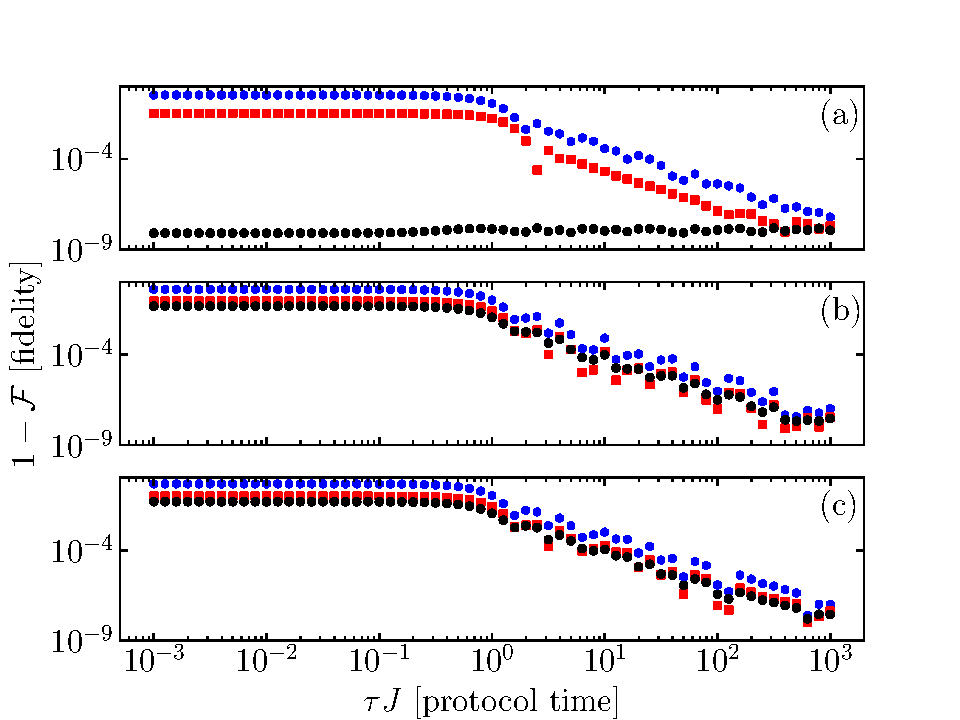
\includegraphics[width=0.49\columnwidth]{IsingVarCDPlots.pdf}
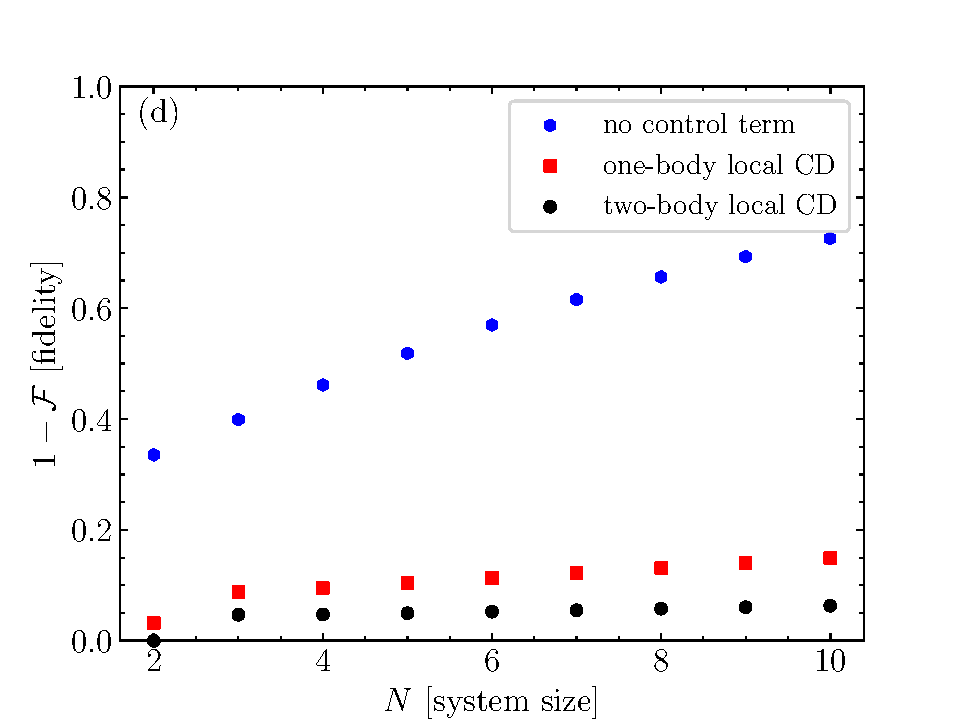
\includegraphics[width=0.49\columnwidth]{IsingNPlot.pdf}
\caption{Implementation of local CD in the Ising spin model. The case of \steve{no control term(s) being} implemented (blue) is compared to implementing one-body local CD (red) and two-body local CD (black). (a-c) The achieved fidelity ($1-\mathcal{F}$) for different total protocol times for (a) $N=2$, (b) $N=3$, and (c) $N=4$ spins. Note, for the case of (a) $N=2$ the two-body local CD gives unit fidelity to below single precision. (d) The achieved final fidelity for a fixed total time, $T=0.01 J^{-1}$, for various system sizes showing the saturation of the fidelity for the one and two-body implementations.}
\label{fig:figvarcd}
\end{figure}

We now turn to a concrete example of the implementation of variational CD in the Ising model. We will consider a system described by Hamiltonian~\eqref{eq:IsingNonIntegrable} with the following parameters
\begin{equation}
    J(\lambda) = J \ , \: Z(\lambda) = J \ , \: X(\lambda) = 2J\lambda \ , \nonumber
\end{equation}
with $\lambda$ being the time-dependent linear function
\begin{equation}
    \lambda(t) = \frac{t}{T} \,
\end{equation}
with $t$ going from $0$ to $T$ where $T$ is the total driving time. This allows us to explore both the adiabatic $T \gg J^{-1}$ and diabatic $T \ll J^{-1}$ regimes. First, we look to confirm that the variational CD terms are correctly derived by considering the case of $N=2$ in Fig.~\ref{fig:figvarcd}(a). Indeed, we observe that for all total driving times, $T$, the fidelity is perfect to single precision, whereas the one-body corrections only compensate some transitions, bringing the fidelity to $\sim\!0.9$. We note here, that there are limited other states for any excited dynamical state to populate with the Hilbert space consisting of only four states, as a result, the bare dynamical protocol with no variational CD still has an overlap of $\sim\!0.6$ with the ground state. Moving to larger systems of $N=3$ and $N=4$ sites in Fig.~\ref{fig:figvarcd}(b) and (c) we observe a clear decrease in the impact of variational CD to only two-body terms. This should be expected as the exact CD will include up to three- and four-body terms in the respective cases. The improvement that two-body variational CD can deliver in these larger systems is still substantial compared to the bare dynamical protocol, showing the utility of low-order variational CD when possible. In Fig.~\ref{fig:figvarcd}(d) we investigate the scaling of the fidelity for the bare and variational CD protocols for a fixed time $T=0.01J^{-1}$. We also briefly note that this approach of variational CD can be enhanced via the introduction of control fields \cite{COLD_PRXQ, morawetz2024efficient}, thus combining the methodologies described in this section with that of Sec.~\ref{sec:QOC}.

\iffalse
We will take as an example a two-spin quantum model with the Hamiltonian
\begin{equation}\label{eq:Htwospin}
    H_0(\lambda) = -2J \sigma_1^z \sigma_2^z - h \sum_{j=1}^{2} \sigma_j^z + 2h\lambda \sum_{j=1}^{2} \sigma_j^x 
\end{equation}
with $\lambda$ being the time-dependent driving field. While this two-spin model could be solved in a rather straightforward fashion to determine the exact CD term in Eq.~\eqref{HCD}, it will serve well as an intuitive example of the approach of variational CD.

Let us consider a scenario where our Hamiltonian is that of Eq.~\eqref{eq:Htwospin} but we are only able to introduce control fields that are entirely local in the spin basis, i.e., only one-body terms. We then would like to know an approximate CD which minimises the adiabatic transitions and to find this we will follow the approach outlined in Sec.~\ref{sec:varcd}. First, we will take as an ansatz for the approximate adiabatic gauge potential all possible one-body terms
\begin{equation}
    A_\lambda = \sum_{j=1}^{2} \left( \alpha \sigma_j^y + \beta \sigma_j^x + \gamma \sigma_j^z \right),
\end{equation}
with the aim being to determine the optimal coefficients $\alpha$, $\beta$, and $\gamma$. Before moving further forward it is useful to write out the commutation rules 
\begin{eqnarray}
    \left[d A, B \right] & = & d \left[A, B \right] \nonumber\\
    \left[A, B + C\right] & = & \left[A, B \right] + \left[A, C\right] \nonumber\\
    \left[ A, BC \right] & = & B \left[ A, C \right] +  \left[ A, B \right] C \nonumber\\
    \left[ AB, C \right] & = & A \left[ B, C \right] +  \left[ A, B \right] B \nonumber
\end{eqnarray}
with $A,B,C$ being operators and $d$ a scalar, and the commutator relations for the Pauli matrices
\begin{eqnarray}
    \left[ \sigma_j^x, \sigma_k^y \right] & = & 2 i \sigma_j^z \delta_{j,k} \nonumber \\
    \left[ \sigma_j^y, \sigma_k^z \right] & = & 2 i \sigma_j^x \delta_{j,k}  \nonumber \\
    \left[ \sigma_j^z, \sigma_k^x \right] & = & 2 i \sigma_j^y \delta_{j,k} \nonumber
\end{eqnarray}
with $\delta_{j,k}$ the Kronecker delta, both of which we will use frequently in this section while finding the commutator term in $G_\lambda$ as given in Eq.~\eqref{eq:glambda}. We can then write $G_\lambda$, taking $\hbar=1$, in terms of the Pauli matrices using the known commutation relations as
\begin{eqnarray}
    G_\lambda & = & \partial_\lambda H_0(\lambda) + i \left[ A_\lambda, H_0 \right] = 2h \sum_{j=1}^{2} \sigma_j^x + i \left[ \sum_{j=1}^{2} \left( \alpha \sigma_j^y + \beta \sigma_j^x + \gamma \sigma_j^z \right), -2J \sigma_1^z \sigma_2^z - h \sum_{k=1}^{2} \sigma_k^z + 2h\lambda \sum_{k=1}^{2} \sigma_k^x  \right] \nonumber \\
    & = & 2h \sum_{j=1}^{2} \sigma_j^x - 2 J i \sum_{j=1}^2 \left[ \left( \alpha \sigma_j^y + \beta \sigma_j^x + \gamma \sigma_j^z \right), \sigma_1^z \sigma_2^z  \right] - i h \sum_{j,k=1}^2 \left[ \left( \alpha \sigma_j^y + \beta \sigma_j^x + \gamma \sigma_j^z \right), \sigma_k^z  \right] + 2 h \lambda i \sum_{j,k=1}^2 \left[ \left( \alpha \sigma_j^y + \beta \sigma_j^x + \gamma \sigma_j^z \right),  \sigma_k^x  \right] \nonumber \\
    & = & 2h \sum_{j=1}^{2} \sigma_j^x - 2 J i \sum_{j=1}^2 \left( \alpha \sigma_1^z \left[ \sigma_j^y, \sigma_2^z  \right] + \alpha \left[ \sigma_j^y, \sigma_1^z  \right] \sigma_2^z + \beta  \sigma_1^z  \left[ \sigma_j^x ,\sigma_2^z  \right] + \beta \left[ \sigma_j^x , \sigma_1^z  \right] \sigma_2^z \right) \nonumber \\ & & - i h \sum_{j,k=1}^2 \left( \alpha \left[ \sigma_j^y , \sigma_j^z  \right] + \beta \left[\sigma_j^x, \sigma_k^z  \right] \right) + 2 h \lambda i \sum_{j,k=1}^2 \left( \alpha \left[ \sigma_j^y,  \sigma_j^x  \right] + \gamma \left[ \sigma_j^z,  \sigma_k^x  \right] \right) \nonumber \\
    & = & 2h \sum_{j=1}^{2} \sigma_j^x - 2 J i \left( 2 \alpha i \sigma_1^z \sigma_2^x + 2 \alpha i \sigma_1^x \sigma_2^z - 2 \beta i  \sigma_1^z  \sigma_2^y -2 \beta i \sigma_1^y \sigma_2^z \right) - i h \sum_{j=1}^2 \left( 2\alpha i \sigma_j^x - 2\beta i \sigma_j^y \right) + 2 h \lambda i \sum_{j=1}^2 \left( -2\alpha i\sigma_j^z + 2 \gamma i \sigma_j^y \right) \nonumber \\
    & = & 2 J \left( 2 \alpha \sigma_1^z \sigma_2^x + 2 \alpha \sigma_1^x \sigma_2^z - 2 \beta  \sigma_1^z  \sigma_2^y -2 \beta \sigma_1^y \sigma_2^z \right) + \left( 2 h + 2 \alpha h \right) \sum_{j=1}^{2} \sigma_j^x + \left( 2 \beta h - 4 \gamma h \lambda \right)  \sum_{j=1}^{2} \sigma_j^y + 4 h \lambda \alpha \sum_{j=1}^{2} \sigma_j^z.
\end{eqnarray}
The action, Eq.~\eqref{eq:AGPaction}, then follows as 
\begin{eqnarray}
    S  (A_\lambda) & = & \Tr \left[G_\lambda^2 (A_\lambda) \right] \nonumber \\
    & = & 32 J^2 \alpha^2 - 32 J^2 \beta^2  + 2 \left( 2 h + 2 \alpha h \right)^2  + 2 \left( 2 \beta h - 4 \gamma h \lambda \right)^2 + 32 h^2 \lambda^2 \alpha^2. \label{eq:2action}
\end{eqnarray}
We can then find the minimum of the action with respect to each parameter of our ansatz to define a system of equations to be solved for the approximate CD. By taking the partial derivatives of Eq.~\eqref{eq:2action} we obtain
\begin{eqnarray}
    \frac{\partial S(A_\lambda)}{\partial \alpha} & = & 64 J^2 \alpha + 8 h \left( 2 h + 2 \alpha h \right) + 64 h^2 \lambda^2 \alpha = 0 \nonumber \\
    \frac{\partial S(A_\lambda)}{\partial \beta} & = & - 64 J^2 \beta + 8h \left( 2\beta h - 4\gamma h \lambda \right) = 0 \nonumber \\
    \frac{\partial S(A_\lambda)}{\partial \gamma} & = & 16 h \lambda \left( 2 \beta h - 4 \gamma h \lambda \right) = 0 \nonumber
\end{eqnarray}
From $\frac{\partial S(A_\lambda)}{\partial \gamma}$ it can be seen that $\gamma = \beta / 2 \lambda$, which can then be subbed into the equation $\frac{\partial S(A_\lambda)}{\partial \beta}$ to give $\beta=0$ and therefore $\gamma=0$. This is not surprising as the eigenstates of Hamiltonian~\eqref{eq:Htwospin} are real and we would therefore expect the CD term to be entirely imaginary. This means that any term that contributes to the adiabatic gauge potential needs to have an odd number of $\sigma^y$ operators. From $\frac{\partial S(A_\lambda)}{\partial \alpha}$ we can then find that
\begin{equation}
    \alpha = -\frac{h^2}{4J^2 + h^2 + 4 h^2 \lambda^2},
\end{equation}
giving an approximate CD term of
\begin{equation}
    H_\text{CD} = - \dot{\lambda} \frac{h^2}{4J^2 + h^2 + 4 h^2 \lambda^2} \sum_{j=1}^2 \sigma^y_j.
\end{equation}

We can continue the approach of variational CD for other, more complicated, ansatze, e.g., in the two-spin model we can take as an ansatz
\begin{equation}
     A^{(2)}_\lambda = \alpha \sum_{j=1}^2 \sigma_j^y +  \gamma (\sigma_1^x \sigma_{2}^y + \sigma_1^y \sigma_{2}^x) +  \zeta (\sigma_1^z \sigma_{2}^y + \sigma_1^y \sigma_{2}^z),
\end{equation}
for which we can follow the same steps to obtain the coefficients $\alpha$, $\gamma$, and $\zeta$. We will leave simplifying the commutators as an exercise for the reader and simply state the resulting set of coupled equations to be solved
\begin{equation}
    \begin{pmatrix}
2\left( 4 h^2 \lambda^2 + 4 J^2 \right) & -8Jh\lambda & -8Jh \\ 
-4Jh \lambda &  \left(  4 h^2 \lambda^2 + 4h^2 \right) & -6 h^2 \lambda \\
-8 Jh & 12 h^2 \lambda & 2 \left(16 h^2 \lambda^2 + J^2 + h^2 \right)
\end{pmatrix}
\begin{pmatrix}
\alpha \\ \gamma \\ \zeta
\end{pmatrix}  = 
\begin{pmatrix}
-2h^2 \\ 0 \\ 4hJ
\end{pmatrix}.
\end{equation}
\callum{I could do all this as well? Will be an even longer bunch of algebra though and it does not require the ability to do anything different from the above derivation}\steve{I think this is fine ``as an exercise".} As this model can only have up to 2-body terms, $A^{(2)}_\lambda$ will give the exact CD but its form could also be used in other Ising models, e.g., on a periodic or finite chain.

\callum{To do: Add plot and discussion of the 1-body and 2-body variational CD.}
\fi

\subsection{Experimental implementations of counterdiabatic driving}
The first experimental demonstrations of such shortcuts to adiabaticity (STA) were performed using trapped Bose-Einstein condensates (BECs)~\cite{STAExp2011, CDExp2012}. In particular, control of the LZ model was achieved using a BEC trapped in an optical lattice and an effective two level system corresponding to Eq.~\eqref{eq:LZham} was accessed, in quasi-momentum space, by accelerating the gas~\cite{CDExp2012}. In this setting the exact CD dynamics, Eq~\eqref{HCD_LZ}, can be achieved in two ways: either directly introducing a second optical lattice that induces the required control field or by making a suitable transformation to the Hamiltonian, in effect absorbing the control field into modulations of the bare Hamiltonian parameters. The latter approach being clearly more experimentally preferable as it requires the manipulation of only a single optical potential. Indeed performing such a transformation to achieve the control is characteristic of many experimental realisation of STA protocols~\cite{CDExp2016a, CDExp2016b, CDExp2017}. The realised protocol was shown to be remarkably robust. Subsequently control of the LZ model was demonstrated in another experimental platform consisting of a single nitrogen-vacancy (NV) centre in diamond, where the effective two-level system was achieved by driving a particular subspace spanned by states of the electron spin~\cite{CDExp2013}. This implementation allowed to demonstrate the remarkable speed up that can be attained with CD driving, achieving an improvement of between 2 and 3 orders of magnitude. 

Counterdiabatic techniques have since been applied to more complex settings starting with three-level systems where CD control can significantly speed up stimulated Raman adiabatic passage protocols~\cite{CDExp2016a, CDExp2017, CDExp2022}, continuous variable control of a trapped ion~\cite{CDExp2016b}, and superconducting Xmon set ups to achieve high fidelity quantum gates~\cite{CDExp2018a} and characterising the thermodynamics of the control protocol~\cite{CDExp2018b}. The energetics of STA protocols has been recently explored in the context of the Landau-Zener model, Eq.~\eqref{HCD_LZ}, using a single trapped $^{40}$Ca$^+$ ion~\cite{STAExp2024} in order to experimentally demonstrate the tradeoff between resource consumption and achievable control~\cite{CampbellDeffnerPRL}.

Approximate CD driving has been demonstrated in controlling transport of population in a synthetic lattice of momentum states in ultracold ${}^{87}$Rb with a two orders of magnitude improvement in population transfer \cite{meier2020counterdiabatic} and in ground state preparation in a nuclear-magnetic-resonance setup \cite{zhou2020experimental}. The commutator exapnsion form of the AGP has led to the developlment of a new family of variaitional quantum algorithms, so-called CD Quantum Approximate Optimisation Algorithm (QAOA) \cite{wurtz2022counterdiabaticity,Chandarana2022digitized} which has been implemented on current hardware, including examining potential applications in protein folding~\cite{Chandarana2023digitized} and finance~\cite{Hegade2022portfolio}.